\documentclass[lettersize,journal]{IEEEtran}
\usepackage{cite}
\usepackage{amsmath,amssymb,amsfonts}
\usepackage[linesnumbered,ruled]{algorithm2e}
\usepackage{graphicx}
\usepackage[utf8]{inputenc}
\usepackage{multicol} 
\usepackage{multirow} 
\usepackage{booktabs}  
\usepackage{threeparttable}  
\usepackage{array}
\usepackage{textcomp}
\usepackage{stfloats}
\usepackage{url} 
\usepackage{caption}
\usepackage{verbatim}
\usepackage{subcaption}
\usepackage{bbding}
\usepackage{textcomp}
\usepackage{xcolor}
\usepackage{graphicx}
\usepackage[caption=false,font=normalsize,labelfont=sf,textfont=sf]{subfig}
\def\BibTeX{{\rm B\kern-.05em{\sc i\kern-.025em b}\kern-.08em
    T\kern-.1667em\lower.7ex\hbox{E}\kern-.125emX}}
\usepackage{amsmath,amsfonts}
\usepackage{array}
\usepackage[caption=false,font=normalsize,labelfont=sf,textfont=sf]{subfig}
\usepackage{textcomp}
\usepackage{stfloats}
\usepackage{url}
\usepackage{verbatim}
\usepackage{graphicx}
\usepackage{cite}
\usepackage{xcolor}
\hyphenation{op-tical net-works semi-conduc-tor IEEE-Xplore}
\captionsetup[subfigure]{font={small,rm}}
\begin{document}

\title{A Model-Agnostic Spatio-Temporal Prediction Framework for Traffic Flow}

\author{Yucen Gao,
        Guorun Huang,
        Bokai Lin,
        % Jun Fang,
        Xiaofeng~Gao*,~\IEEEmembership{Senior~Member,~IEEE}, % <-this % stops a space 
        Bin Wang,
        Xiaochun~Yang,~\IEEEmembership{Senior~Member,~IEEE},
        Guihai~Chen,~\IEEEmembership{Fellow,~IEEE}%
\thanks{Xiaofeng Gao is the corresponding author.}
\thanks{Yucen Gao, Bin Wang, and Xiaochun Yang are with the Software College of Northeastern University, Shenyang, China, 110819 (e-mail: \{gaoyucen, binwang, yangxc\}@mail.neu.edu.cn).

Guorun Huang, Xiaofeng Gao and Guihai Chen are with Shanghai Key Laboratory of Scalable Computing and Systems, School of Computer Science, Shanghai Jiao Tong University, Shanghai, China, 200240 (e-mail: huang.guor@northeastern.edu, \{gao-xf, gchen\}@cs.sjtu.edu.cn).

% Jun Fang is with Didi Global Inc., Beijing, China, 100190 (e-mail: fangjun@didiglobal.com).
}
}

% The paper headers
\markboth{Journal of \LaTeX\ Class Files,~Vol.~14, No.~8, August~2021}%
{Shell \MakeLowercase{\textit{et al.}}: A Sample Article Using IEEEtran.cls for IEEE Journals}

\IEEEpubid{0000--0000/00\$00.00~\copyright~2021 IEEE}
% Remember, if you use this you must call \IEEEpubidadjcol in the second
% column for its text to clear the IEEEpubid mark.

\maketitle

\begin{abstract}
Traffic flow prediction is a critical issue in transportation engineering and presents distinct challenges when handling large-scale datasets in the real world. Traffic flows in the same city show a rich variety of characteristics at different times and locations. Existing complex spatio-temporal forecasting paradigms, which use the same parameters to fit traffic sequences with varying spatio-temporal features, tend to train an average performance model over different time series. This approach greatly reduces their accuracy when applied to larger road networks. Moverover, the significant differences in traffic data distribution from one city to another can also pose great challenges. The same model may be excellent for one city and mediocre when applied to another. To this end, we propose a \textbf{Meta} Backbone Agnostic \textbf{S}patio-\textbf{T}emporal \textbf{C}lustering Framework for Traffic Forecasting on Large-Scale Road Networks named \textbf{MetaSTC}. We tackle the disparities of spatio-temporal features of traffic flow through a spatio-temporal clustering-based strategy. We design meta-learner for large-scale road network by incorporating a cluster-aware memory unit that dynamically extracts the shared context information across roads in the same sub-task. In this way the model is able to represent task-specific details with a simpler model and makes quick and accurate predictions. Our paradigm is backbone-agnostic that can be combined with different traffic prediction models, solving the problem caused by the difference in data distribution. Extensive experimental results conducted on real-world traffic datasets demonstrate the high accuracy and computational efficiency of our model over state-of-the-art approaches. 
\end{abstract}

\begin{IEEEkeywords}
Traffic Flow Prediction, Backbone Agnostic, Clustering, Meta-Learning, Spatio-Temporal Data Mining.
\end{IEEEkeywords}

\section{Introduction}
\IEEEPARstart{T}{he} traffic flow prediction problem is a crucial endeavor within the field of transportation engineering, focusing on the prediction of temporal sequences that represent future traffic conditions. \textcolor{blue}{As illustrated in Figure\ref{fig:application}, traffic flow prediction plays a pivotal role in optimizing the functioning of transportation systems such as traffic management strategies, congestion mitigation efforts, and efficient scheduling practices\cite{DBLP:journals/suscom/Medina-SalgadoS22}.}

\begin{figure}[tbp]
\centering
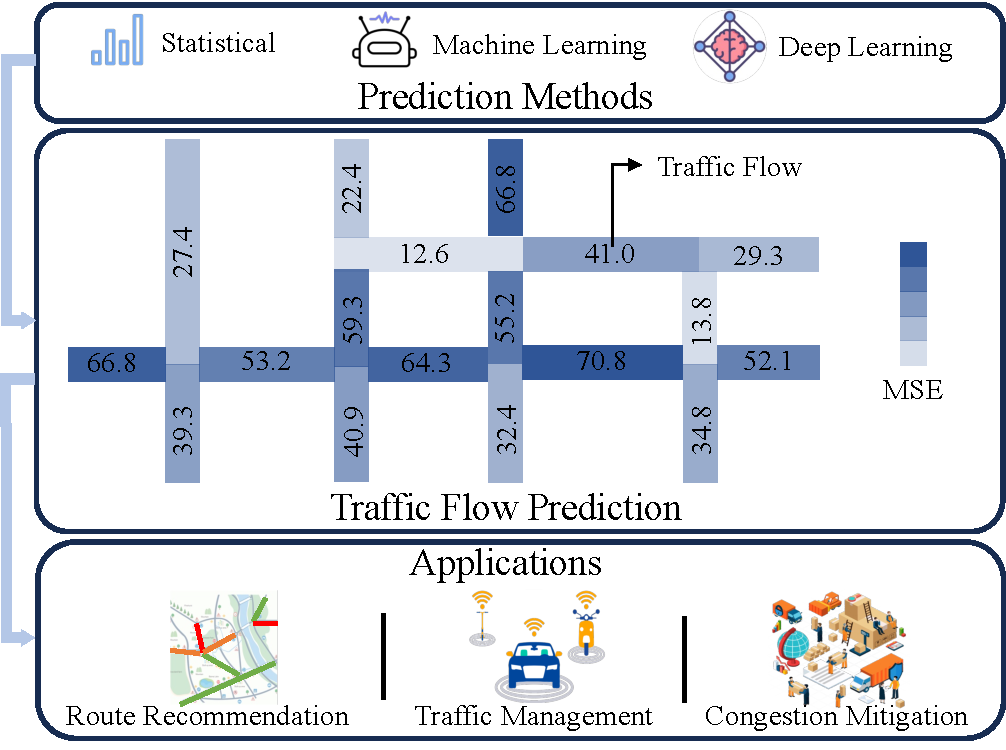
\includegraphics[width=0.45\textwidth]{figure/application.pdf}
\caption{\textcolor{blue}{The Process of Traffic Flow Prediction.}}
\label{fig:application}
\end{figure}



The field of traffic flow prediction dates back to 1959 by H Greenberg~\cite{greenberg1959analysis}. Over the years, there has been continuous research in the field of traffic prediction, covering a wide range of methods including statistical approaches, traditional machine learning techniques, and more recently, deep learning models. However, existing works face challenges in terms of precision and applicability to \textbf{real-world datasets}. We outline these challenges as follows:

% challenges

\IEEEpubidadjcol

\textbf{Challenge 1: Complex Traffic Mode}
Traffic flow exhibits inherent time dependence with cyclic fluctuations occurring on daily, weekly, and yearly scales. Spatial disparities can be ascribed to various factors such as differences in economic development levels, area topography, and planning strategies.  Figure~\ref{fig:diverse} shows the differences in traffic patterns for three roads from different locations. The flow sequences of the three roads can be seen to show a daily regularity but with different patterns of increase and decrease. Road 2 shows a peak during the day and decreases in flow as the night goes on, while the remaining two do the opposite. The mean values of flows for the first road and the second road are close to and higher than the rest. It is difficult to fit all the roads in the network with the same set of parameters.


\textbf{Challenge 2: Large Scale Dataset}
Due to the inextricable relationship between the traffic prediction problem and real-world scenarios, We should consider the feasibility and effectiveness of model design applied to large-scale datasets of real scenarios. In reality, a mid-sized city requires traffic forecasting including approximately hundreds of service areas and thousands of roadways for each area~\cite{largest}.  Figure~\ref{fig:large} demonstrates the relationship between the monitoring data used for actual downstream forecasting and the public datasets used for traffic forecasting research. The current test results on previous small public datasets are not necessarily applicable to larger datasets. Test results on large-scale public data~\cite{largest} have also shown that previous work has degraded performance on large-scale datasets. The performance of the model in the face of large-scale datasets is yet to be explored.

% Furthermore, timely adaptability is critical in traffic flow forecasting. Without the ability to quickly update predictions during emergencies like traffic accidents, authorities may not be able to respond promptly, leading to prolonged congestion and safety hazards. Therefore, having a system that can dynamically update and adjust traffic flow predictions in real-time is essential to effectively handle unforeseen events and minimize their impact. Considering lightweight models becomes crucial to ensure timely and efficient traffic flow predictions.



\textbf{Challenge 3: Diverse Spatio-Temporal Scenarios}
For different road scenarios, the traffic flow pattern laws show different data distributions. For example, in metropolitan areas, traffic near business districts will have significant peaks in commuting time intervals while these traffic modes do not apply in the countryside. Figure~\ref{fig:scene} shows different scenarios such as cities, villages, campuses, and resorts. Under different data scenarios, the performance of one model varies greatly, and it is difficult to have a generalized model to fit all the datasets with different data distributions~\cite{survey}. 

\color{blue}
To address the aforementioned challenges, we develop a \textbf{Meta} \textbf{S}patio-\textbf{T}emporal \textbf{C}lustering Learning Paradigm named \textbf{MetaSTC}. Our model integrates two components: the spatio-temporal representation clustering module and the spatio-temporal meta-learning module. 


\begin{figure}[htbp]
\centering
\begin{minipage}[t]{0.44\textwidth}
\centering
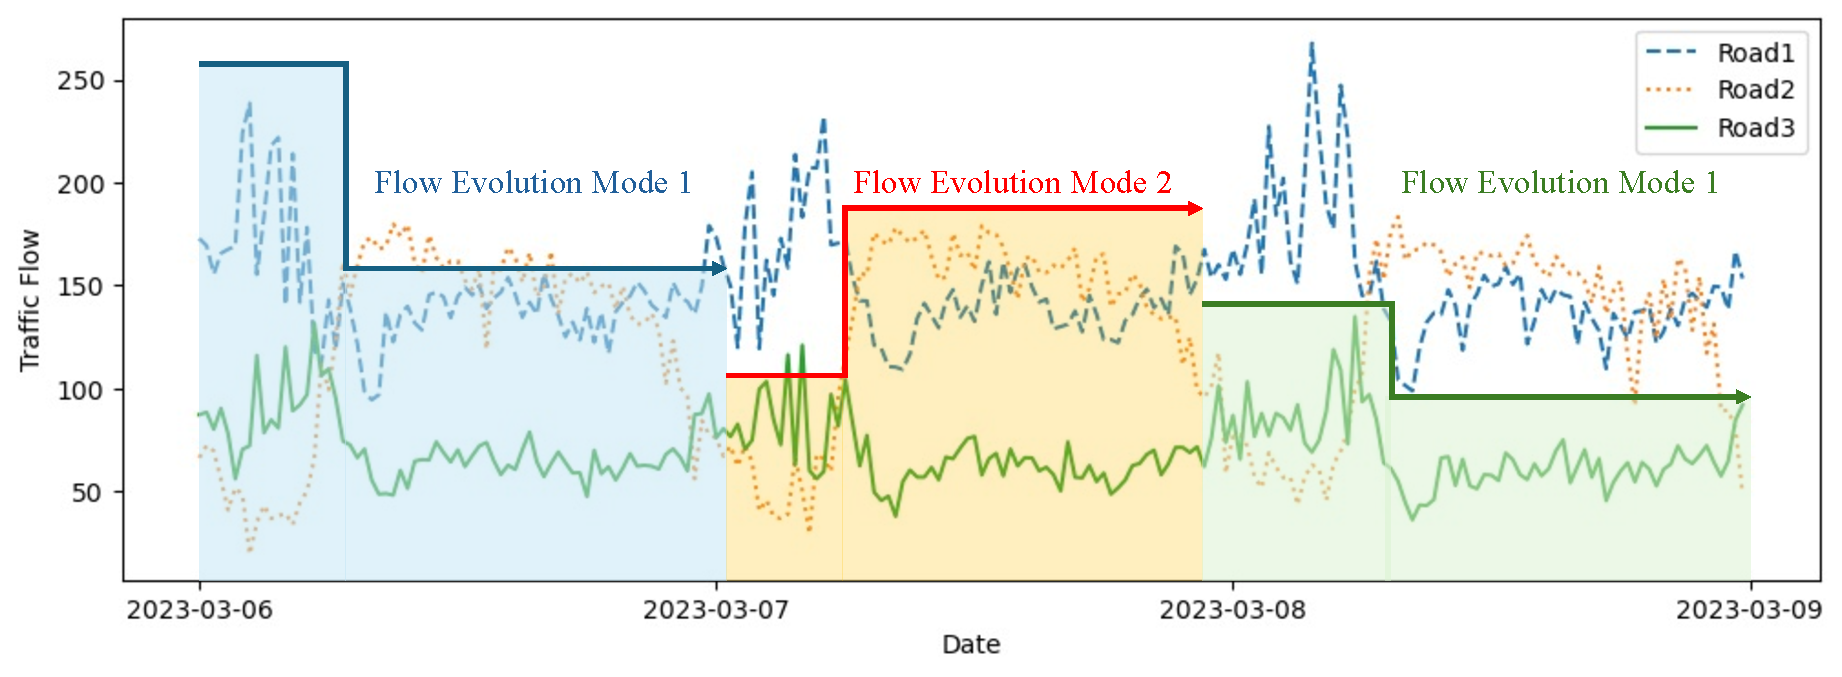
\includegraphics[width=7.5cm]{figure/Mode_Vis_2.pdf}
\subcaption{Complex ST Correlations}
\label{fig:diverse}
\end{minipage}
\begin{minipage}[t]{0.22\textwidth}
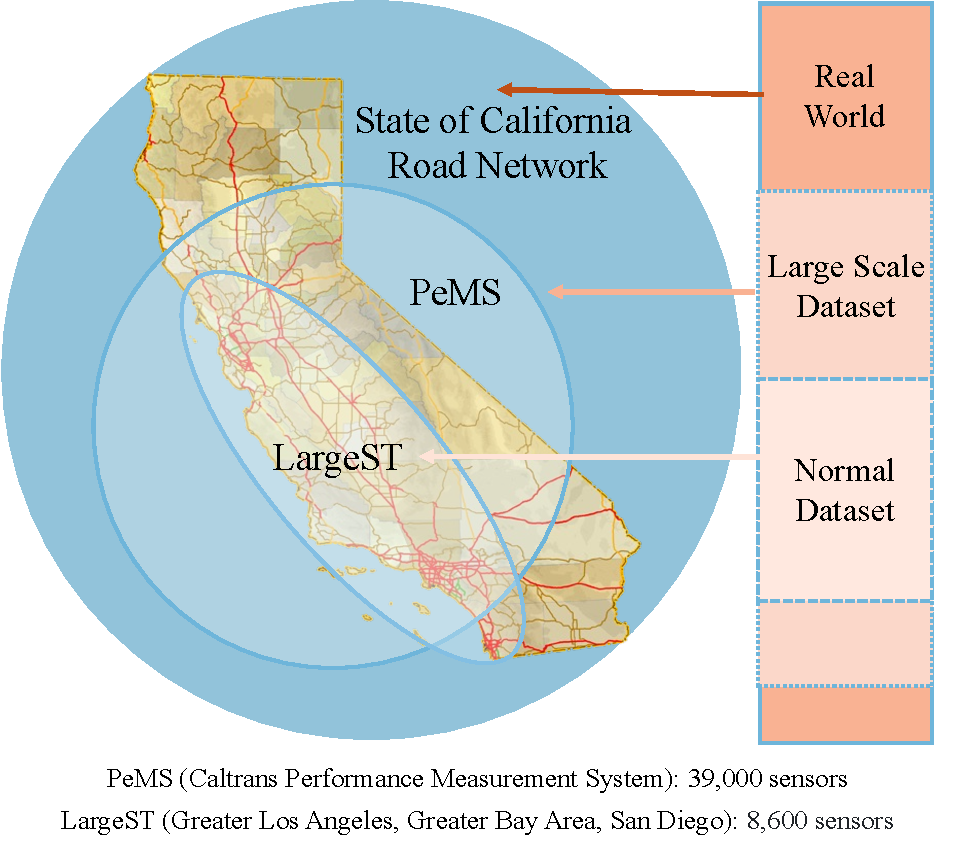
\includegraphics[width=3.6cm]{figure/California_Data.pdf}
\centering
\subcaption{Large Scale Dataset}
\label{fig:large}
\end{minipage}
\begin{minipage}[t]{0.22\textwidth}
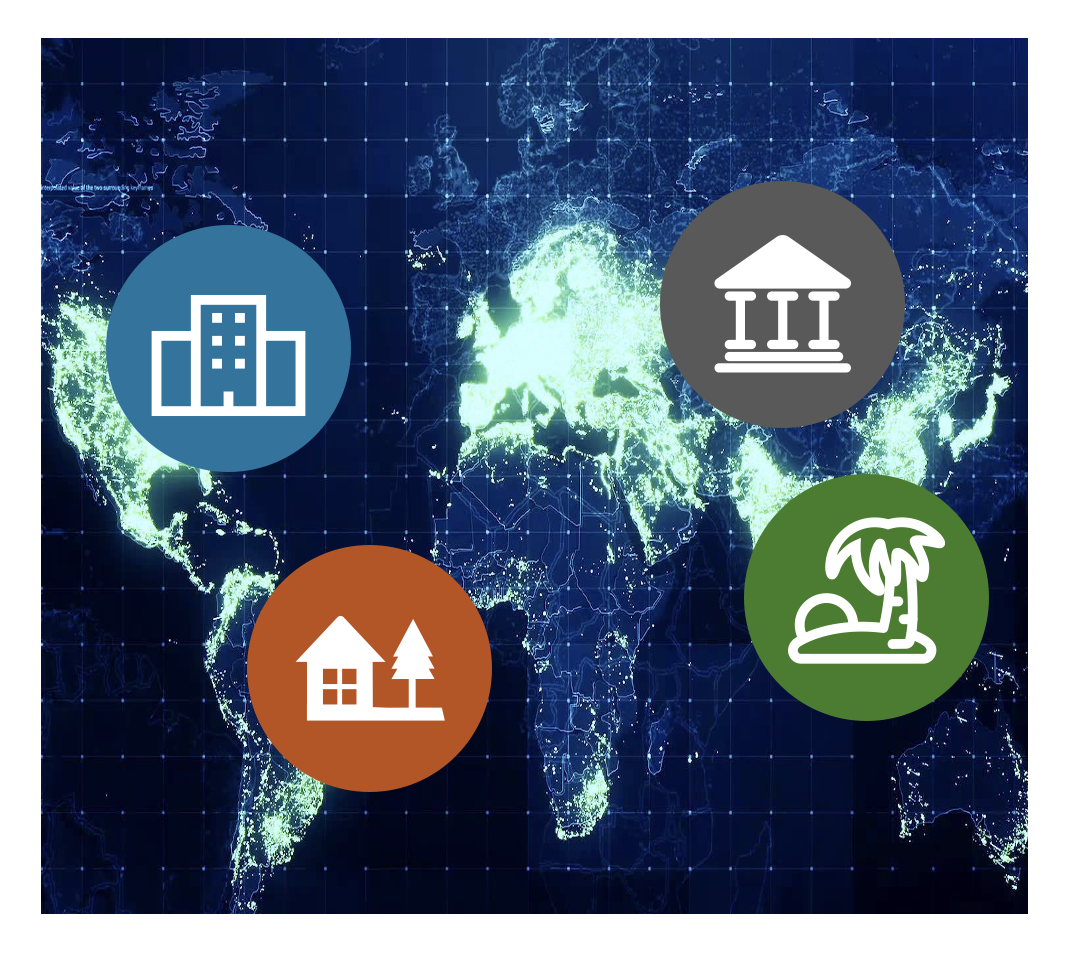
\includegraphics[width=3.6cm]{figure/c3.png}
\centering
\subcaption{Diverse Scenarios}
\label{fig:scene}
\end{minipage}
\\
\caption{Challenges of Traffic Flow Prediction.}
\label{fig:challenge}
\end{figure}


Gabriel Cirstea et al.~\cite{DBLP:conf/icde/CirsteaYGKP22} mentioned that a shared network for all the road networks forces the learned parameters to represent an “average” of the traffic patterns among all traffic flow series.  Considering the complex traffic mode in road network (mentioned in \textbf{Challenge 1}), they used spatial-aware modeling where different model parameters can be used for modeling time series from different locations. But fitting every feature pattern on the road network with a separate parameter again brings excessive training time as well as the problem of overfitting. In order to reduce the variability of feature distribution in the dataset, we include K-Means method to group together roads into clusters. Previous clustering based methods for traffic prediction (e.g. Hwang Kuo et al.~\cite{kuo_adaptive_2001}) lack the discussion of spatio-temporal features. We design a spatio-temporal gating unit to capture spatio-temporal contextual information and apply the clustering based on obtained spatio-temporal representation. For the road nodes within the same cluster, the differences between them are relatively small because they share similar spatio-temporal patterns. 


As mentioned above, state-of-the-art models have demonstrated exceptional performance on small-scale datasets (e.g. Pemsd~\cite{PeMSD}) by considering the dynamic characteristics of spatial topology, but their complex designs prevent them from scaling to larger datasets~\cite{largest}. More complex network structures require higher computational resources (e.g. running memory, training time) and limit the size of the batch size with the same computational resources, which brings about instability in training. To enhance the applicability of the model to real-world datasets (\textbf{challenge 2}), we design a meta-learner that refines global models with specific subtasks rather than training a mega-scale model. The meta-learner makes it possible to represent task-specific details with a simpler model, and reduces the likelihood of its overfitting. Meta-learning can be seen as an advanced form of transfer learning that transfers not only knowledge but also learning strategies to improve overall stability and performance through information sharing between tasks~\cite{DBLP:journals/corr/FinnAL17}.

Previous work applying meta-learning to solve traffic flow prediction problems~\cite{pan_urban_2019}~\cite{zhang_efficient_2022}~\cite{wang_deep_2022} lacked experimental validation on large-scale datasets and didn't put any restrictions on choosing subtasks. We improved the meta-learner by developing a contextual memory unit. Building upon the earlier established categories, our contextual memory unit extracts sub-task-related information for model prediction. The meta-learner learns information from the single road scope, from the subtask scope, and from the entire dataset scope which improves the prediction performance on large-scale datasets.


In order to cope with the great variability of traffic flow pattern laws in different road scenarios \textbf{(challenge 3)}, our framework adopts backbone agnostic modularity design, which allows key components such as the prediction backbone network, feature fusion module, etc. to be independently upgraded or replaced, and facilitates the rapid iteration of the model structure according to the scenarios.

\color{black}
In all, our contributions can be summarized as follows.
		
\begin{enumerate}
\item  We are at the forefront of traffic flow forecasting in practical scenarios by introducing a groundbreaking lightweight backbone agnostic paradigm that makes predictions on real-world datasets. We compared in Table~\ref{tab:adv} the differences between the baseline models to highlight the advantages of MetaSTC.

% clus
\item A new encoding method is proposed to extract the spaio-temporal features to obtain spatio-temporal representation with rich context information.

% meta
\item We introduce a spatio-temporal clustering-based meta-learner which includes contextual information to each meta-task for more accurate and efficient prediction.

% exp
\item We conduct extensive experiments on real-world traffic flow datasets. Our MetaSTC model shows high accuracy and computational efficiency.

\end{enumerate} 

\begin{table}[!t]
    \centering
    \caption{Advantages of MetaSTC compared to other traffic flow prediction methods.}
    \label{tab:adv}
    \setlength{\tabcolsep}{1mm}
    \resizebox{0.5\textwidth}{!}{%
    \begin{tabular}{ccccc}
    \toprule  
    Advantages   & Spatio-Temporal Correlation   &  Divide-and-Rule &   Backbone Agnostic \\
    \midrule
    TimesNet~\cite{DBLP:conf/iclr/WuHLZ0L23} & \XSolidBrush   & \XSolidBrush  & \XSolidBrush   \\
     STGCN~\cite{stgcn}  & \Checkmark  & \XSolidBrush   & \XSolidBrush   \\
 ASTGCN~\cite{ast-gcn} & \Checkmark  & \XSolidBrush   & \XSolidBrush   \\
     AGCRN~\cite{10.5555/3495724.3497218} & \Checkmark  & \XSolidBrush   & \XSolidBrush   \\
     PDFormer~\cite{DBLP:conf/aaai/JiangHZW23}  & \Checkmark  & \XSolidBrush   & \XSolidBrush   \\
      DCRNN~\cite{metrla}  & \Checkmark  & \XSolidBrush   & \XSolidBrush   \\
  Graph Wavenet\cite{graphwave}  & \Checkmark  & \XSolidBrush   & \XSolidBrush   \\
   ST-WA~\cite{DBLP:conf/icde/CirsteaYGKP22}  & \Checkmark  & \XSolidBrush   & \Checkmark   \\
    \textbf{MetaSTC(ours)}   & \Checkmark  & \Checkmark   & \Checkmark   \\
    \bottomrule
    \end{tabular}%
    }
\end{table}



\begin{figure*}[htbp]
\centering
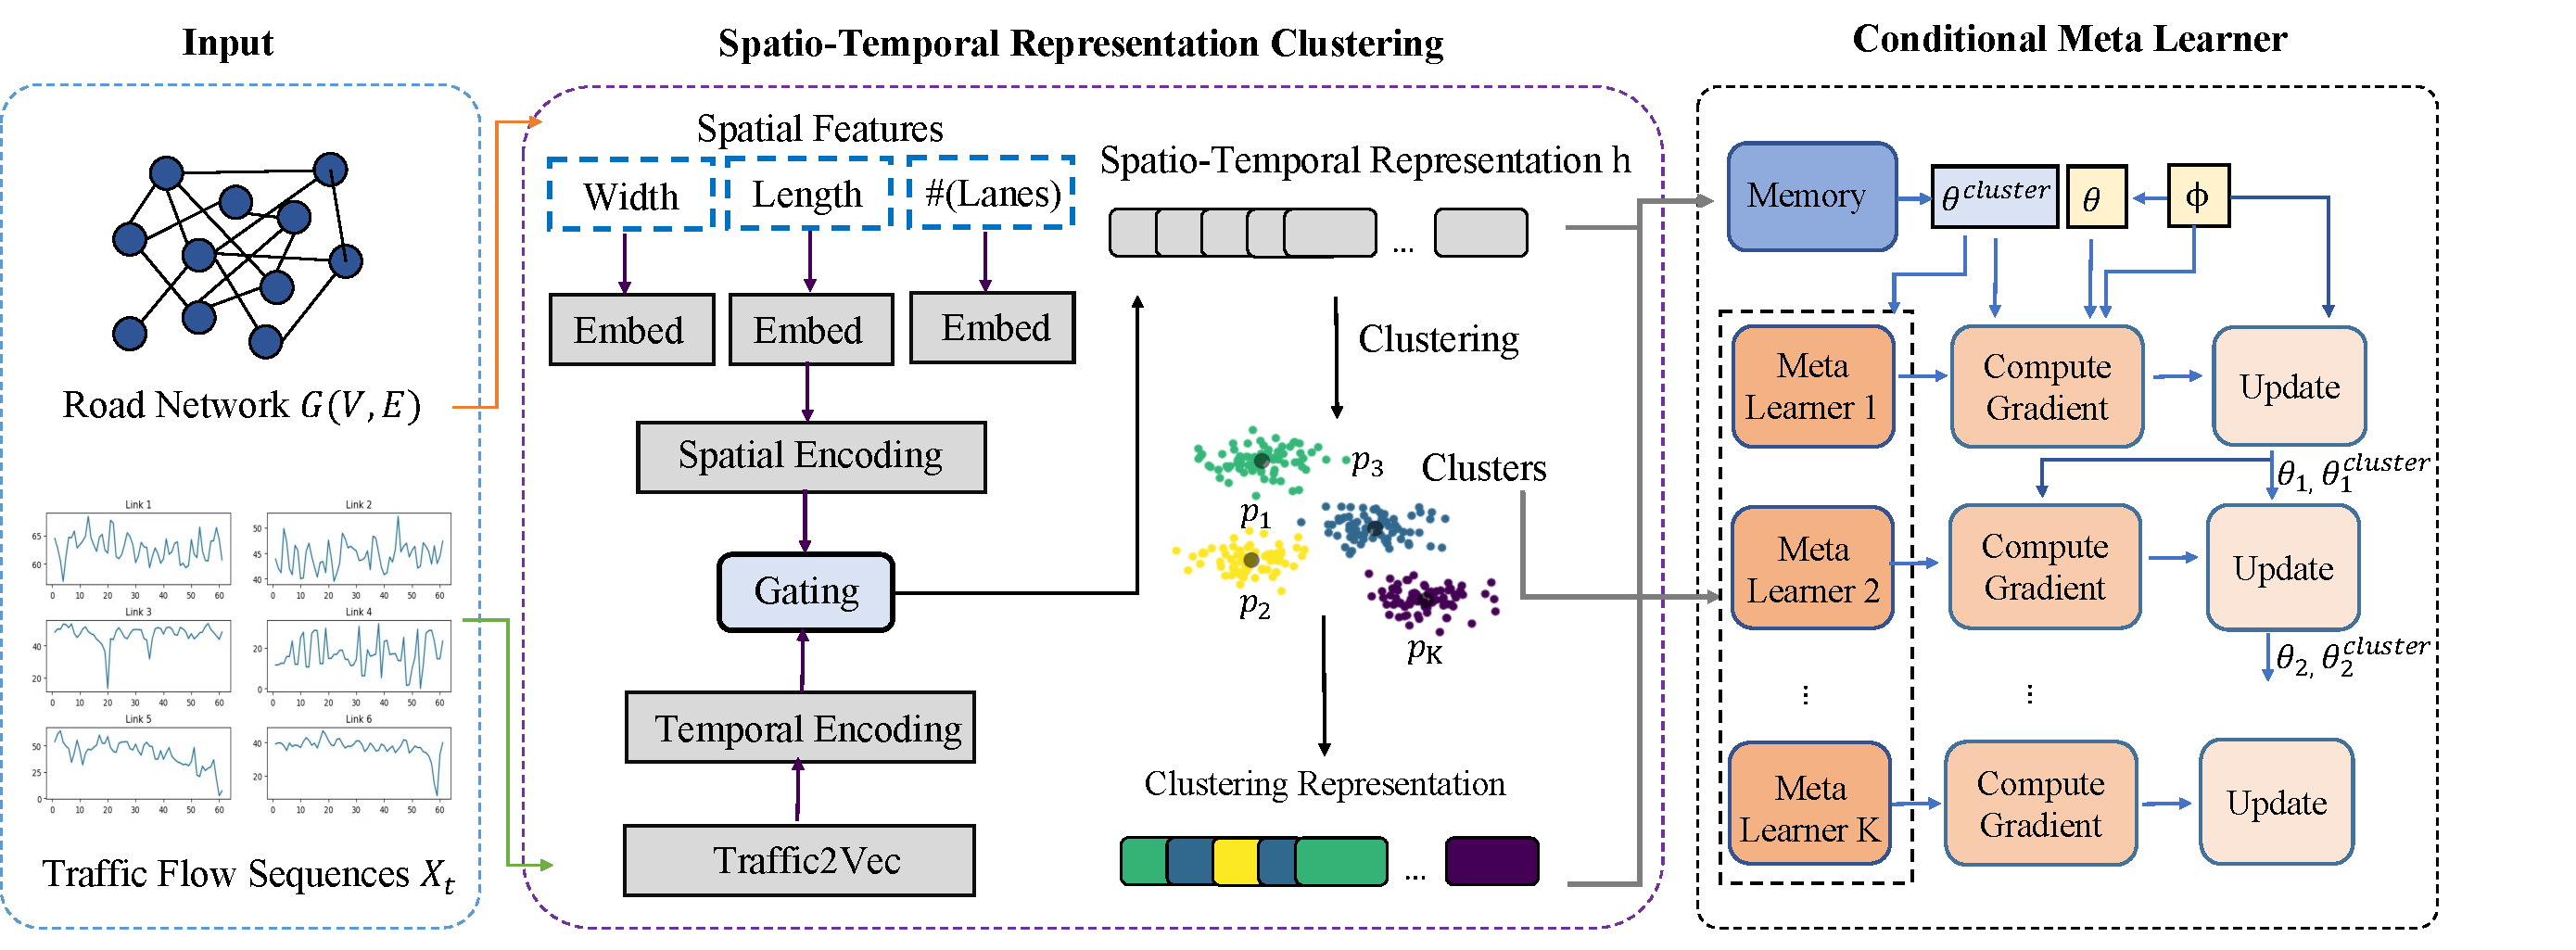
\includegraphics[width=\textwidth]{figure/framework.pdf}
\caption{The Framework of Metastc. Our model contains two components: a spatio-temporal representation clustering module and a meta-learning module.}
\label{fig:framework}
\end{figure*}
\section{Preliminaries and Problem Formulation}
In this section, we first define the key concepts for modeling the flow of traffic on the road and then formulate our problem. 

\textbf{Traffic Flow Sequence}
We define the traffic network as a directed graph $G = (V, E)$, where $V$ is the set of nodes that represents the intersections of the roads, and $E$ is the set of edges that represents the roads. At a specific time stamp $t$, a traffic flow sequence $X_t$ represents a $L$ long historical traffic flow data on the entire road network. Specifically, $X_t = \{x_{t-L},\cdots, x_{t-1}\}$, where $x_i$ represents the traffic flow at the historical time stamp $i$ for all roads. In our discussion, we use the speed of the traffic to represent the traffic flow.


\textbf{Traffic Flow Prediction Problem}
Given time stamp $t$, the traffic flow prediction problem aims to predict the future traffic flow for all roads. More specifically, provided the traffic flow sequence $X_t$, a prediction model $p$ predicts the traffic flow for the next few time stamps $p(X_t) = \{\hat{x}_{t+1}, \cdots, \hat{x}_{t+P}\}=\{\hat{x}\}_{t+1}^{t+P}$, where $P$ denotes the prediction horizon. The goal is to minimize the cumulative loss $L = \sum_{t = L+1}^T \mathcal{L}(\{\hat{x}\}_{t+1}^{t+P}, \{x\}_{t+1}^{t+P})$, where $T$ is the total number of predicted steps, and $\mathcal{L}(\cdot, \cdot)$ can be any loss function such as MAE and RMSE.


% \begin{figure*}[htbp]
% \centering
% 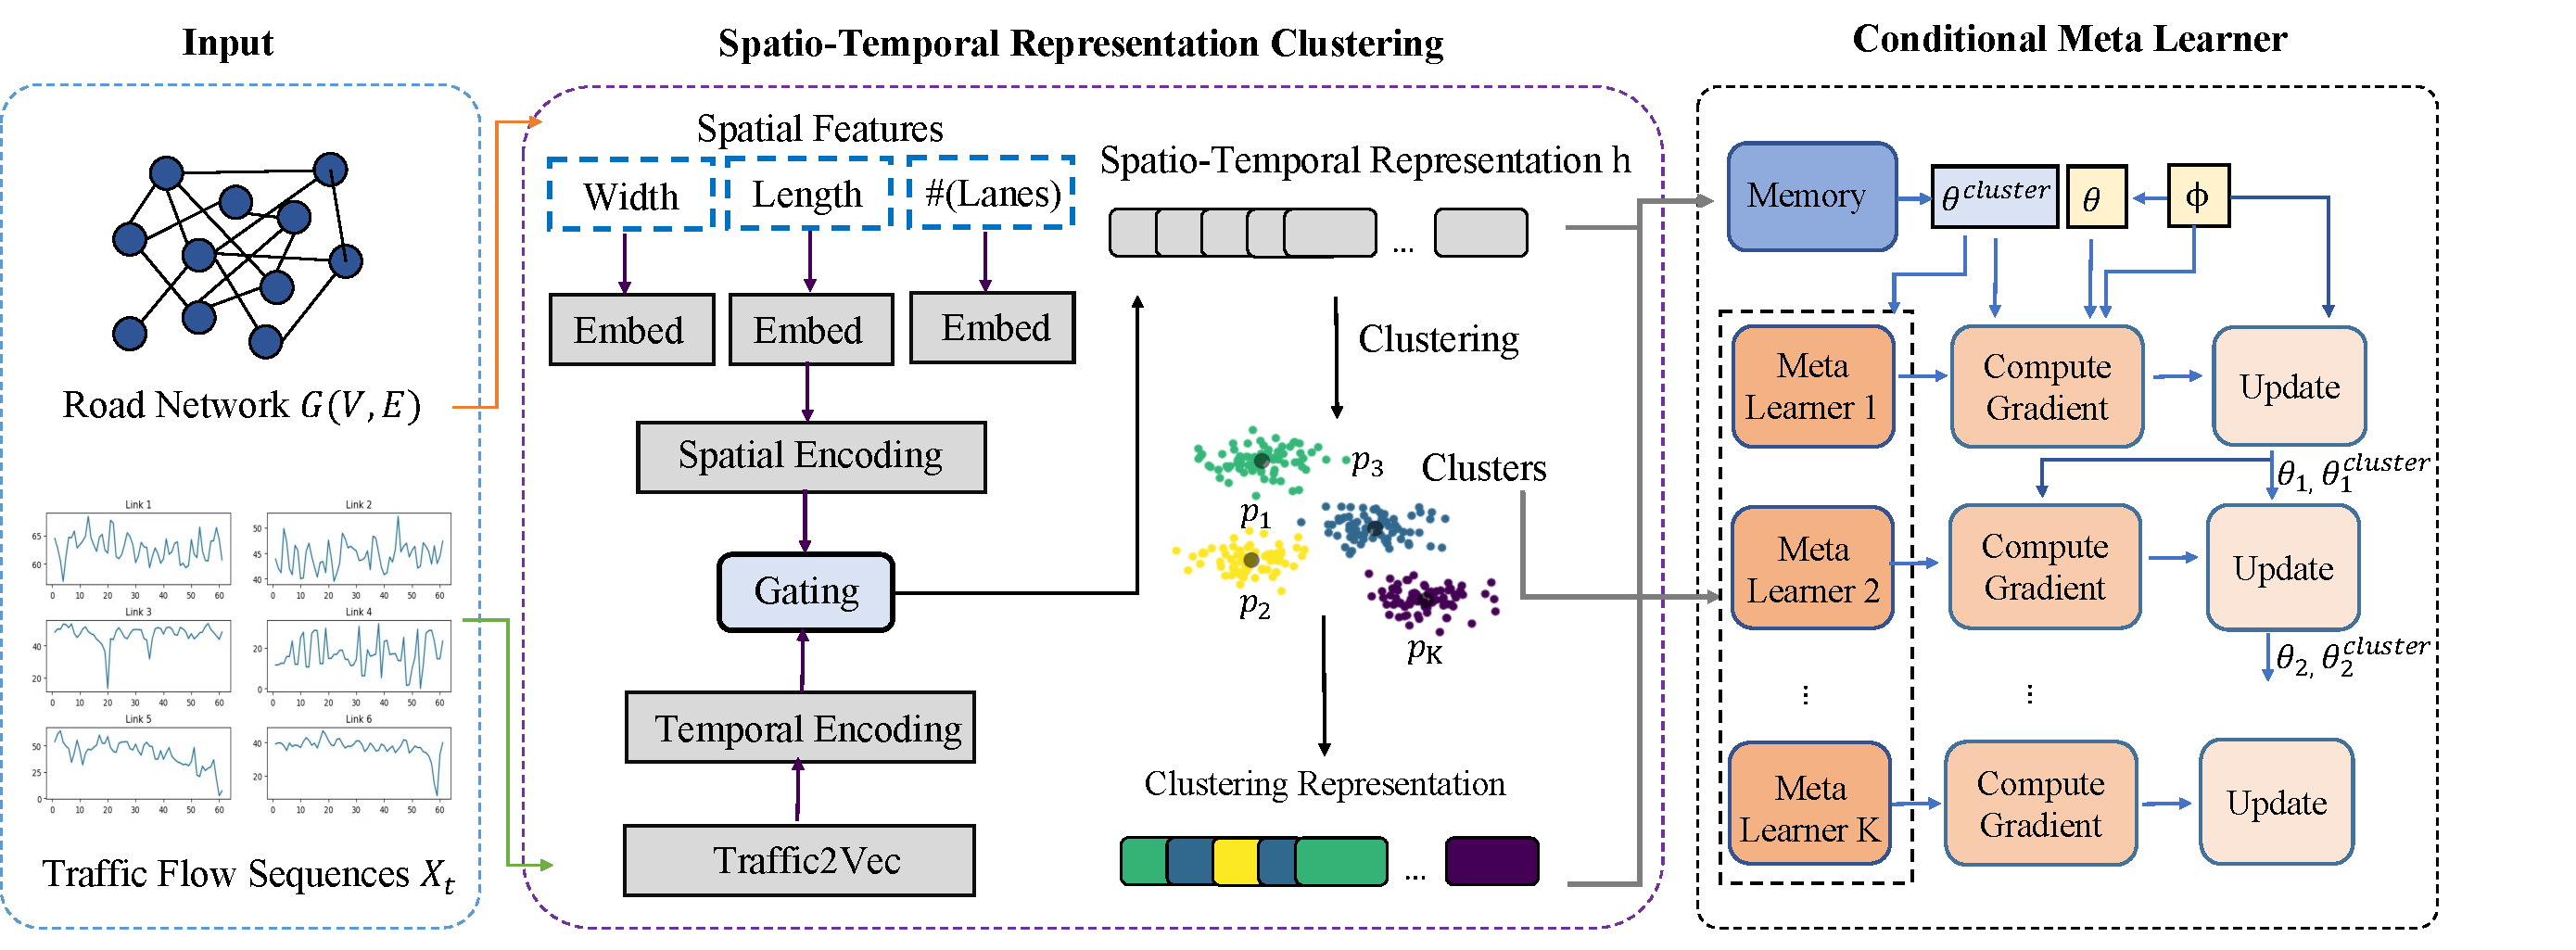
\includegraphics[width=0.9\textwidth]{figure/framework.pdf}
% \caption{The Framework of Metastc. Our model contains two components: a spatio-temporal representation clustering module and a meta-learning module.}
% \label{fig:framework}
% \end{figure*}


\section{Methodology}

Our MetaSTC paradigm is composed of two major modules: the road clustering module and the meta traffic forecasting module. Our overall framework is outlined in Figure~\ref{fig:framework}. \textcolor{blue}{The clustering module reduces the variability of spatio-temporal patterns in the same subtask and meta-learning can adaptively adjust training for different subtasks. The proposed flow forecasting model is customized for each cluster, i.e., the parameters in the neural network are the same for the roads within the same cluster and vice versa.}

\subsection{Spatio-Temporal Representation Clustering}

As \textbf{challenge 1} describes, traffic flow inherently possesses temporal and spatial dependencies. In order to better capture the cross-region traffic flow transfer patterns, we propose a spatio-temporal representation learning method for roads. \textcolor{blue}{In addition to the dynamic traffic flow patterns, we consider as well as static attributes of road segments that influence the actual travel flow such as the road index (roadID), road level (roadLevel), and the number of lanes (laneNum). Table~\ref{tab:feature} depicts all the spatio-temporal features in MetaSTC. We train a gating mechanism to embed the dynamics and interactions amongst roads. Finally, we cluster roads with similar patterns.}

\begin{table*}[!t]
    \centering
    \caption{Spatial and Temporal Features.}
    \label{tab:feature}
    \setlength{\tabcolsep}{2mm}
    \resizebox{0.95\textwidth}{!}{%
    \begin{tabular}{cccc}
    \toprule  
       & Feature   & Description  &  Possible Range of Values  \\
    \midrule
   Temporal & MonthID & An identifier for each month in a year & Integer from 1 to 12\\
    & WeekID & An identifier for each day of the week & Integer from 1 to 7 \\
     Spatial & RoadID & The identifier of the sensor & A number with 6 to 9 digits\\
      & RoadLevel & The hierarchical level of road & Primary, Secondary, Tertiary \\
     & Lat & The latitude of road & Real number between -90 and 90 \\
      & Lng & The longitude of road & Real number between -180 and 180 \\
      & LaneNum & The number of lanes & Integer from 1 to 8 \\
    & Width & The width of road  & Real number (unit: meters) \\
    & Length & The length of road & Real number (unit: meters) \\
    & Direction & The direction of the highway & North (N), South (S), East (E), West (W) \\
    \bottomrule
    \end{tabular}}
    \end{table*}

\textbf{Temporal Features} To capture the various changing temporal patterns mentioned above, we start with a standardized approach to reprocess traffic flow data. Standardization helps to remove the scale and shift differences that might exist in the data, making it more suitable for further analysis. 

As mentioned in the introduction, traffic flow data exhibit strong periodicity on a day and week scale. Recognizing these clear cyclical trends is critical for accurate traffic prediction and analysis. Therefore, we encode a time point $t$ with a combination of linear and periodic functions that encapsulate these two essential temporal dimensions. The encoding is formulated as
\begin{gather}
    \text{Traffic2Vec}(X_t) = 
    \begin{bmatrix} 
    \text{Traffic2Vec}(t)  \ 
    \vdots \ 
    \text{Traffic2Vec}(t+T) \ 
    \end{bmatrix}\\
    \text{Traffic2Vec}(t) = [w_0 t + b_0, \sin(w_d t + \phi_1), \sin(w_w t + \phi_2)].
\end{gather} 
Here, $w_0 t + b_0$ represents the linear component and  $\sin$ terms encode the daily and weekly cycles respectively, \textcolor{blue}{where $w_d$ denotes for the daily frequency ($\frac{2\pi}{24}$) and $w_w$ denotes for the weekly frequency ($\frac{2\pi}{7 \times 24}$). The $\phi$ terms are learnable parameters that denote phase shifts, allowing our model to adjust to the specific temporal dynamics of the traffic flow.
After computing the temporal encoding, we apply a dense layer, to further process the sequence
\begin{equation}
h_t = \text{Dense}(X_t,\text{Traffic2Vec}(X_t))
\end{equation}
where Dense represents the dense layer with its own set of learnable weights. By constructing the temporal hidden state in this way, the model can capture both the explicit temporal encoded patterns and the implicit patterns which increases the interpretability of models.}

\textbf{Spatial Features} Spatial attributes of road segments also play an important role in traffic flow prediction. Part of the attributes, such as the road index, road level, and the number of lanes, are categorically valued and thus cannot be fed into the model directly. It is generally computationally expensive to tackle these features by the one-hot encoding. To solve this problem, we embed the discrete features into a low-dimensional space to seek compact representations as well as to share similar patterns across different road segments. The embeddings are concatenated to form the spatial hidden state 
\begin{equation}
    h_s = M_{index} \oplus M_{level} \cdots \oplus M_{lane}
\end{equation}
where $ M_{index}, M_{level}, M_{lane}$ are trainable embedding matrices and $\oplus$ represents the concatenate operation.

\textbf{Spatio-Temporal Gating Unit} 
\textcolor{blue}{The integration of spatial and temporal features in traffic flow prediction requires a mechanism capable of modeling their complex, nonlinear interactions. Simply concatenating or adding these features, as done in traditional approaches, risks losing critical contextual information due to the heterogeneous nature of traffic data across time and space. In our context, the spatio-temporal gating unit is designed to dynamically weigh the contributions of spatial and temporal hidden states based on their relevance to the prediction task. This approach aligns with the principle of attention in sequence modeling, where the model learns to focus on salient features. Mathematically, the gating vectors $G_s$ and $G_t$ (defined below) act as adaptive filters, modulating the influence of $h_s$ and $h_t$ through a sigmoid activation. This ensures that the final representation $h$ preserves both spatial topology and temporal periodicity while mitigating noise from irrelevant features, a critical requirement given the cyclic yet variable nature of traffic patterns (Challenge 1).}

We want to find a way to transform the spatial and temporal features into a format that captures the essential spatio-temporal context information. Instead of simply adding or concatenating, here we design a gating unit linking spatial and temporal representations to obtain the hidden states used for clustering. This allows the model to control the flow of information more flexibly by learning weights to understand complex nonlinear relationships to better capture the interactions between different features. As a result, the model can automatically determine the level of contribution of each hidden state based on a specific task, which is more flexible and adaptable. The formulas are as follows
\begin{align}
    G_s &=  \text{sigmoid}(W_{ss}h_s+W_{ts}h_t+b_s)\\
    G_t &=  \text{sigmoid}(W_{st}h_s+W_{tt}h_t+b_t)\\
    h &=  [G_s \odot h_s || G_t \odot h_t].
    \label{equ:h}
\end{align}


Here, $G_s$ and $G_t$ are gating vectors for spatial and temporal states, respectively. \textcolor{blue}{$W_{ss}$ and $W_{tt}$ are the self-gating weight matrices for the spatial and temporal states. In contrast, $W_{ts}$ and $W_{st}$ are cross-gating weight matrices that allow each state to influence the gating of the other. The biases $b_s$ and $b_t$ adjust the activation of the gates.}

The final hidden state $h$ combines the gated spatial and temporal states, preparing the features for clustering and further analysis. This unit enables the model to dynamically prioritize salient spatio-temporal features for improved predictive performance. We train all the parameters during the global updating process of the flow forecasting task.

\textcolor{blue}{From a signal processing perspective, the gating unit can be viewed as a dynamic filter that disentangles the periodic components of traffic flow (e.g., daily and weekly cycles) from spatially-driven variations (e.g., road hierarchy and topology). This is particularly advantageous in traffic data, where temporal periodicity is often corrupted by spatial heterogeneity, such as differing peak hours across urban and rural roads (Challenge 1). By assigning learnable cross-gating weights \(W_{ts}\) and \(W_{st}\), the model effectively performs a form of feature selection, amplifying relevant spatio-temporal interactions while suppressing noise, akin to adaptive filtering in time-series analysis. This theoretical underpinning ensures that the resulting representation \(h\) is not only expressive but also robust to the multi-scale dependencies inherent in large-scale traffic networks.}

\textbf{Spatio-Temporal Road Network Clustering}
As is mentioned in \textbf{challenge 1}, traffic flow patterns vary greatly from time to time and from location to location, while a unified model uses a single set of parameters over all the roads, and thus has limits in capturing data variability over large regions. Therefore, we thought of training multiple sub-regions separately. We conduct K-Means++ over the spatio-temporal embeddings by the representation learning model to obtain the clustering over the road network.

\begin{algorithm}[htbp]
    % \SetAlgoLined
    \KwIn{Traffic flow sequences $X_t$, Road features $f_s$,  Number of clusters $K$} 
    \KwOut{Spatio-Temporal representation $h$, Cluster centroids $p_1, p_2, \cdots, p_K$}
    \ForEach{$x_{i,t} \in X_t$}{ 
        $h_{i,s} \gets \text{Spatio Encoder}(f_{i,s})$\;
        $h_{i,t} \gets \text{Temporal Encoder}(x_{i,t})$\;
        $h_i \gets \text{Gating}( h_{i,s} , h_{i,t})$\;
    }
    \textbf{Initialize} $p_1, p_2, \cdots, p_K $ \textbf{at random};\;
    \While{not converged}{ 
        \ForEach{$x_{i,t} \in X_t$}{ 
            \For{$j = 1$ \KwTo $K$}{
                $\mathbb{P}_j(i) \gets \frac{\text{Distance}(h_i - p_j)^2}{\sum \text{Distance}(h_i - p)^2} $\;
            }
        }
        \textbf{Sample} $p_1, p_2, \cdots, p_K $ \textbf{from} $X \sim \mathbb{P}(X)$\;
    }
    \caption{\textcolor{blue}{Spatio-Temporal Representation Clustering}} 
    \label{algo:representation_learning} 
\end{algorithm}

\textcolor{blue}{The process of the representation clustering module is described in Alg.~\ref{algo:representation_learning}.} When encountering a new road, we can rapidly obtain representation and assigned tasks. 

\subsection{Spatio-Temporal Meta Learner}
\textcolor{blue}{Traffic flow prediction on large-scale datasets demands a model that can generalize across diverse road segments while adapting to their unique spatio-temporal characteristics. Traditional deep learning models, trained on a single global parameter set, often struggle to capture this heterogeneity, resulting in suboptimal performance on unseen scenarios (Challenge 2). To overcome this, we adopt a meta-learning paradigm, rooted in the concept of ``learning to learn'', which enables rapid adaptation to new tasks by leveraging prior knowledge. Unlike standard transfer learning, meta-learning optimizes an initial parameter set that can be fine-tuned efficiently for specific subtasks---in our case, clusters of roads with similar patterns. This approach is theoretically grounded in Model-Agnostic Meta-Learning (MAML)~\cite{DBLP:journals/corr/FinnAL17}, where a meta-learner minimizes the expected loss across tasks via second-order optimization. By integrating clustering with meta-learning, we ensure that the model not only captures global traffic dynamics but also tailors predictions to local contexts, enhancing scalability and robustness on real-world datasets. The subsequent design of our cluster-aware memory unit builds upon this foundation, embedding task-specific priors into the learning process.}

As \textbf{challenge 2} mentioned, due to the inextricable relationship between the traffic prediction problem and real-world scenarios, models that can be applied to large-scale datasets of real-world scenarios are more meaningful. \textcolor{blue}{To address this, we proposed a spatio-temporal meta-learning module that aims to better adapt the prediction model to large-scale datasets. In urban areas, the temporal patterns, characteristics of locations, and the mutual relationship of roads are diverse.} So far, we have divided the entire road network into multiple categories of smaller sizes based on the spatio-temporal features of each road. In this spatio-temporal meta-learning module, we use the meta-learner to train unique model parameters for each category. \textcolor{blue}{The separation of learning of category priors makes it possible to represent road-specific details with a simpler model within the smaller dataset. Each time we initial from the global parameters based on the previous pre-trained tasks.}

\textcolor{blue}{The synergy of clustering and meta-learning in our framework further optimizes the bias-variance trade-off, a key concern in statistical learning for heterogeneous datasets. By partitioning the road network into clusters with similar spatio-temporal patterns, we reduce the variance within each subtask, allowing the meta-learner to focus on task-specific adaptations rather than fitting a single, overgeneralized model. This aligns with the principle of task distribution modeling in meta-learning, where the meta-learner implicitly learns a prior over a family of related tasks (i.e., clusters) rather than individual data points. Consequently, the model achieves improved generalization on unseen roads by leveraging shared knowledge across clusters, while the localized fine-tuning mitigates overfitting—a critical advantage when scaling to thousands of roads with diverse distributions (Challenge 2).}

\color{blue}

\textbf{Cluster-aware Memory Unit}
To accommodate the unique characteristics of roads influenced by various contextual factors, it is impractical to use a one-fits-all approach with global parameters for traffic flow prediction. Recognizing the impact of road diversity, we have formulated a cluster-aware contextual memory unit $M_c$ that preserves distinct parameters for the predictive layer tailored to different road clusters. This memory unit is responsible for dispensing personalized initial parameters for each road, drawing on a similarity score computed by a prescribed algorithm.

Upon completion of a clustering operation, we ascertain the centroid of each cluster $p_j$, with $j$ indexing the clusters. We then define a similarity score, represented as $a$ to quantify the closeness of a given road's features to the cluster centroid. The similarity score $a_j^k$ between road $j$ and cluster $k$ can then be recalculated using a softmax function as 
\begin{equation}
     a_j^k = \frac{\exp(p_k \cdot h_j)}{\sum_{i=1}^{K} \exp(p_i \cdot h_j)}
\end{equation} 
where $K$ represents the total number of cluster and $h_j$ reflects the hidden state of $j$-th road calculated by equation~\ref{equ:h}. Specifically, we retrieve the parameter matric $M_{j,c}$ for the $j$-th road $ M_{j,c} = a_j^k \cdot M_c $.

In the spirit of LSTM~\cite{lstm}, our memory unit integrates a reset gate and an update gate to manage its parameters effectively. As the training process unfolds, the memory unit retrieves and updates the initial parameters $M_c$ as
\begin{align}
r_t & = \sigma(W_r \cdot (a_j^k \otimes M_{j,c}) + b_r) \\
u_t & = \sigma(W_u \cdot  (a_j^k \otimes M_{j,c}) + b_u) \\
\tilde{M_c} & = \tanh(W_c \cdot (r_t \odot (a_j^k \otimes M_{j,c})) + b_c) \\
M_c & = (1 - u_t) \otimes M_c + u_t \otimes \tilde{M_c}
\end{align}

In these equations, $r_t$ is the reset gate at time $t$, $u_t$ the update gate, $h_{t-1}$ the parameter state at the previous time step, and $\sigma$ denotes the sigmoid activation function. The weight matrices $W_r$, $W_u$, and $W_c$, along with their corresponding bias terms $b_r$, $b_u$, and $b_c$, adjust the gates and parameter updates accordingly. $M_c$ is then utilized by the meta learner to initialize the local parameters at the current timestep. This results in a contextually informed and adaptive prediction model capable of yielding more accurate and reliable traffic flow estimations.

\color{black}

\textbf{Local Update}
In traditional meta model such as MAML~\cite{DBLP:journals/corr/FinnAL17}, we split the traffic flow sequences into a training set $\mathcal{D}_{train}$ and a testing set $\mathcal{D}_{test}$ and partition the training set as the support set and query set. The support set is to adapt the model's parameters, and the query set is to evaluate how well the adapted model can generalize to new data. Our target is to find optimal parameters such that for each specific task, it produces task-specific parameters on all the tasks and helps the meta-model achieve the lowest error on their validation data. This can be expressed as
\begin{equation}
    \Theta^* = arg min_{\Theta} \frac{1}{N} \sum_i \mathcal{L}(\text{meta-model}(\mathcal{D}_{i,test} ; \Theta_i) , \mathcal{D}_{i,test}).
\end{equation}
where $N$ is the number of tasks, and $\Theta$ denotes all the parameters in our meta-learning model, $i$ denotes the $i$-th task. We can bring in any model for sequence prediction to combine with our meta-model. We solved \textbf{challenge 3} with this backbone agnostic design. During the experiments, we tested our paradigm by combining LSTM and FiLM models.

\color{blue}

On this basis, we design our spatio-temporal meta-learner. Our target is to ensure that initial parameters for two roads are similar if they share similar spatio-temporal embeddings. We initialize clustering parameters $\theta^{cluster}$ from the contextual memory unit $M_c$ that are specific to the clustering component of the meta-model. We also have shared parameters $\theta$ that are shared across all roads.  We initialize the local parameters $\theta$ from the global parameters $\Theta$. They capture the common features and patterns that are relevant for all roads. They help improve the prediction accuracy of unique tasks which equals categories in our paradigm. The local learning rate is denoted as $\beta$. We rewrite the local updating process of our meta-learning process as
\begin{align}
\theta_i^{cluster} & \xleftarrow{} \theta_i^{cluster} - \beta \nabla_{\theta_i^{cluster}} \mathcal{L}_{D_s},\\
\theta_i & \xleftarrow{} \theta_i - \beta \nabla_{\theta_i} \mathcal{L}_{D_s}
\end{align}
where $\mathcal{L}_{D_s}$ represents the loss on the support set.

\color{black}

\textbf{Global Update}
\begin{gather}
\Phi \xleftarrow{} \Phi - \gamma \sum \nabla_{\Phi} \mathcal{L}_{D_q}
\end{gather}
where $\mathcal{L}_{D_q}$ represents the loss function on the query set and the global learning rate is denoted as $\gamma$. Both local update and global update are computed via back-propagation. This workflow exhibits high scalability, enabling us to efficiently incorporate new nodes by seamlessly integrating them into meta-tasks and obtaining personalized prediction results.

\section{Experiment}
\label{sec:exp}
In this section, we first introduce the experimental setup including the dataset, running environment, evaluation metrics, baseline methods, and model parameters. \textcolor{blue}{Following that, we will proceed to conduct a series of experiments aimed at addressing the following questions:
\begin{itemize}
\item \textbf{RQ1}: How does MetaSTC perform as compared with state-of-art traffic flow prediction model on real-world large-scale datasets?
\item \textbf{RQ2}: Are the key components in MetaSTC (i.e. clustering module and meta-learning module) necessary for improving performance?
\item \textbf{RQ3}: How does MetaSTC perform as a lightweight backbone agnostic paradigm for temporal models? How do MetaSTC's prediction results assist in reducing cost?
\end{itemize}}

To reproduce our results, we upload our code in an anonymous GitHub repository~\footnote{\url{https://github.com/GaoYucen/MetaSTC}}.

\subsection{Experiment Setting}
\textbf{Datasets}
We use real traffic datasets of two different cities from an anonymous company~\footnote{Because of the double-blind requirement, we hide the company name. This will be made public later.} and two public datasets~\cite{PeMSD}~\cite{largest} for experiments. For traffic data, we take every 5 minutes as a time interval and use the average of the traffic speed data recorded during the 5 minutes as the traffic speed value for the period according to actual industrial customs and requirements~\cite{survey}. Figure~\ref{fig:roadnetworks} presents road networks of various cities. Detailed statistics are presented in Table~\ref{tab:data}. 
\begin{table}[!t]
    \centering
    \caption{Statistics of the Datasets.}
  \label{tab:data}
  \resizebox{0.45\textwidth}{!}{%
  \setlength{\tabcolsep}{3mm}
    \begin{tabular}{lccc}
    \toprule  
    Dataset & $\#$Roads & Time Range \\
  \midrule
    Beijing & 7949 & 2023/01/01-2023/03/31 & \\
    Shanghai & 5144 & 2023/06/01-2023/06/30\\
    PeMS04 & 307 & 2018/01/01 - 2018/02/28 \\
    LargeST & 8600 & 2017/01/01 – 2021/12/31\\
    \bottomrule  
    \end{tabular}}
\end{table}

\begin{figure}[htbp]
\centering
\begin{minipage}[t]{0.2\textwidth}
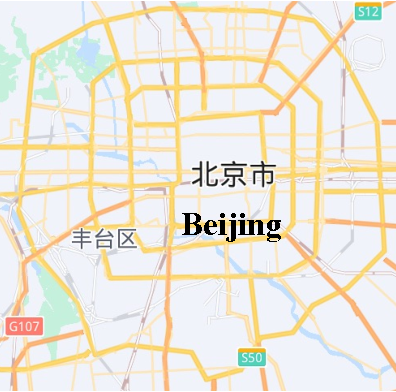
\includegraphics[width=3cm]{figure/beijing.pdf}
\centering
\subcaption{Beijing}
\label{fig:beijing}
\end{minipage}
\begin{minipage}[t]{0.2\textwidth}
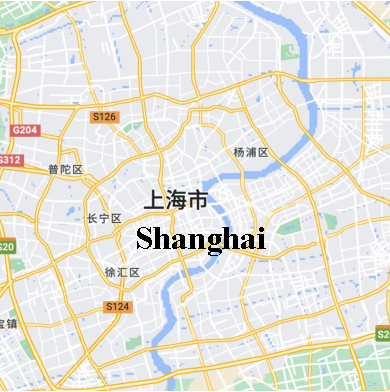
\includegraphics[width=3cm]{figure/shanghai.pdf}
\centering
\subcaption{Shanghai}
\label{fig:shanghai}
\end{minipage}
\\
\begin{minipage}[t]{0.4\textwidth}
\centering
\includegraphics[width=6.7cm]{figure/California.pdf}
\subcaption{California}
\label{fig:california}
\end{minipage}
\caption{Road Networks of Different Cities. We used company-provided data for the first two cities, as well as two publicly available datasets from California traffic data.}
\label{fig:roadnetworks}
\end{figure}


\textbf{Environment and Device Setting}
Our experimental environment is configured with the following specifications: Pytorch 2.10, Python 3.8~(Ubuntu 20.04), and CUDA 11.2. The GPU used for the experiment is the A40 with 48GB memory and a four-way SLI configuration, while the CPU is an AMD EPYC 7543 32-core Processor with 60 vCPUs. The system has a total of 320GB of memory, with a 25GB system disk and a data disk with 50GB of SSD storage, which can be expanded or contracted as required.

 \textbf{Evaluation Metrics:}
We use the Mean Absolute Error~(MAE), Root mean squared error~(RMSE), and the Mean Squared Error~(MSE) for the evaluation of accuracy. Our training loss is according to MSE.

\color{blue}

\textbf{Baselines:}
Considering the limitation of computability as well as the greatness of dataset size, we choose the following models as baselines:
\begin{itemize}
\item Autoregressive Integrated Moving Average model~(ARIMA): ARIMA is a differential integrated moving average autoregressive model~\cite{arima}.

\item LSTM (Long Short-Term Memory): LSTM is a temporal recurrent neural network (RNN). Due to its unique design structure, LSTM is suitable for processing and predicting important events in time series with very long intervals and delays~\cite{lstm}. 

% \item Attribute-Augmented Spatiotemporal
% Graph Convolutional Network~(AST-GCN): AST-GCN models the dynamic and static attributes then encode those factors into the spatio-temporal graph convolution model~\cite{ast-gcn}.
\item Temporal Graph Convolutional Network~(T-GCN): T-GCN is a traffic flow prediction model based on graph convolutional neural network. The time-varying graph-structured traffic flow data is well handled by splitting the time nodes and capturing the relationship of roads with a graph network at each time step.~\cite{tgcn}.

% \item ASTGCN (Attention-based Spatial-Temporal Graph Convolutional Network): ASTGCN is a model that incorporates attention mechanisms to capture the importance of different regions in the graph and temporal dependencies~\cite{astgcn}. 
% \item ASTGNN (Attention-based Spatial-Temporal Graph Neural Network): ASTGNN is a model that extends ASTGCN by introducing gated recurrent units (GRUs) to better capture the temporal dependencies. ASTGNN has state-of-the-art performance in several benchmark datasets, surpassing the other models including ASTGCN~\cite{astgnn}.

\item TimesNet: TimesNet divides complex time changes into multiple intra-periodic and inter-periodic changes, which are embedded into a two-dimensional tensor to realize adaptive discovery of multi-periodicity~\cite{DBLP:conf/iclr/WuHLZ0L23}.

\item DLinear: DLinear first decomposes the input into a trend component by a moving average kernel and a remainder component. Then apply linear layers to each component and at last sum them up to get the final prediction~\cite {aaai/ZengCZ023}.

\item Frequency improved Legendre Memory model~(FiLM): FiLM applies Legendre Polynomials projections to approximate information, uses Fourier projection to remove noise, and adds a low-rank approximation to speed up the calculation process~\cite{nips/ZhouMWW0YY022}.

\end{itemize}

\color{black}


\begin{table*}[!t]
    \centering
    \caption{Performance of MetaSTC and Baselines.}
    \label{tab:comp}
    \setlength{\tabcolsep}{3mm}
    \resizebox{0.8\textwidth}{!}{%
    \begin{tabular}{cccccccc}
    \toprule  
    && \multicolumn{2}{c}{MAE~$\downarrow$} & \multicolumn{2}{c}{MSE~$\downarrow$}  & \multicolumn{2}{c}{RMSE~$\downarrow$}  \\
    & Model & $L=12$  & $L=24$  & $L=12$  & $L=24$   & $L=12$  & $L=24$ \\
    \midrule
    Beijing& ARIMA & 10.607 & 10.757 & 177.101 & 185.531 & 13.308 & 13.633 \\
    &T-GCN & 9.299 & 10.925 & 182.050 & 198.364 & 13.493 & 14.084 \\
    &TimesNet & 3.903 & 4.253 & 36.351 & 40.874 & 6.029 & 6.393 \\
    &DLinear & 4.294 & 4.180 & 38.846 & 38.287 & 6.233 & 6.188 \\
    &LSTM & 4.837 & 4.844 & 46.483 & 46.472 & 6.818 & 6.817 \\
    &FiLM & 3.391 & 3.547 & 28.226 & 29.663 & 5.313 & 5.446 \\
    &MetaSTC+LSTM & 3.534 & 3.710 & 27.433 & 29.040  & 5.238 & 5.343 \\
    &MetaSTC+FiLM & \textbf{3.367}  & \textbf{3.476} & \textbf{26.893} & \textbf{27.527} & \textbf{5.19} & \textbf{5.247} \\
    \midrule
    Shanghai & ARIMA & 9.026 & 9.303 & 134.129 & 142.827 & 11.581 & 11.951  \\
    &T-GCN & 4.340 & 4.365 & 40.692 & 41.525 & 6.380 & 6.444 \\
    &TimesNet & 4.338 & 4.787 & 44.385 & 51.402 & 6.662 & 7.170  \\
    &DLinear & 4.560 & 4.364 & 46.176 & 43.031 & 6.795 & 6.560  \\
    &LSTM & 5.816 & 6.167 & 67.160 & 80.620 & 8.195 & 8.980 \\
    & FiLM & 4.389 & 4.215 & 45.241 & 39.901 & 6.726 & 6.317  \\
    &MetaSTC+LSTM & 4.524 & 4.429 & 42.380 & 40.276 & 6.510 & 6.346  \\
    &MetaSTC+FiLM & \textbf{4.018} & \textbf{4.173 }&\textbf{ 37.076} &\textbf{ 37.992} & \textbf{6.089 }& \textbf{6.164 } \\
    \midrule
    PeMS04 & ARIMA & 10.644 & 10.661 & 160.730 & 163.333 & 12.678 & 12.780 \\
    &T-GCN & 1.973 & 1.384 & 4.309 & 9.840 & 1.807 & 2.145 \\
    &Timesnet & 1.114 & 1.574 & 4.667 & 9.354 & 2.160 & 1.789 \\
    &DLinear & 1.197 & 1.388 & 4.573 & 4.998 & 2.138 & 2.236 \\
    &FiLM & 0.947 & 1.140 & 3.199 & 4.573 & 1.789 & 2.148 \\
    &MetaSTC+LSTM & 1.011 & 1.103 & 3.888 & 4.759 & 1.972 & 2.181  \\
    &MetaSTC+FiLM & \textbf{0.870} & \textbf{0.859} & \textbf{ 2.589} & \textbf{2.360} & \textbf{1.609}& \textbf{1.536}  \\
    
    \midrule
    LargeST & ARIMA & 10.644 & 10.661 & 160.730 & 163.333 & 12.678 & 12.780 \\
    &T-GCN & 6.159 & 5.294 & 64.770 & 55.042 & 8.048 & 7.419 \\
    &TimesNet & 4.729 & 5.089 &49.054 &53.283 &7.004 & 7.299  \\
    &DLinear & 4.975 & 4.798 & 50.074 & 47.204 & 7.076 & 6.871 \\
    &LSTM & 5.934 & 6.142 & 70.606 & 75.824 & 8.403 & 8.708\\
    & FiLM & 4.395 & 4.788 & 43.472 & 48.743 & 6.593 & 6.982  \\
    &MetaSTC+LSTM & 4.644 & 5.032 & 45.520 & 49.102 & 6.747 & 7.007  \\
    &MetaSTC+FiLM &\textbf{ 4.369} &\textbf{ 4.491} & \textbf{43.333 }& \textbf{44.398 }&\textbf{ 6.583 }& \textbf{6.663}\\
    \bottomrule  
    \end{tabular}}
\end{table*}

\textbf{Parameters:}
Referring to public traffic prediction datasets~\cite{PeMSD}, we take 5 minutes as a time step and predict the next $6$ steps from the previous $L$ steps. $L$ is set to 12 and 24. We divide the experimental training set and test set according to $8:2$. Based on the trade-offs between convergence speed and accuracy, we use the Adam optimizer with an early stop when converging. The hyperparameter settings are as follows: The learning rate is set to 0.001, and the number of epochs is set to $1000$. The batch size is set to 64. The dimension of representation is set to $12$. The Euclidean function is chosen as the distance function. The clustering number is set to $5$. The number of layers is set to $3$. 


\subsection{Experiment Results: RQ1}
The MetaSTC model supports combining different traffic flow prediction models. In this section, to balance efficiency and performance, we choose to combine the meta-learning module of our model with the LSTM and FiLM models, respectively. Table~\ref{tab:comp} shows the performance and training time of baseline methods and our proposed MetaSTC model. 



In terms of prediction accuracy, our MetaSTC model achieves the best performance when combined with the advanced deep learning model FiLM. CNN-based deep learning models like TimesNet have generally achieved relatively good performance, which may be attributed to the strong learning ability of deep learning models. 

Spatial-temporal graph neural network-based models combine graph neural networks with multiple temporal learning networks to capture dynamic properties in spatial and temporal dimensions. As the road network data increases, the model complexity as well as the number of parameters increases. \textcolor{blue}{With the same memory resources, we have to reduce the batch size. This makes the training of the model less stable and difficult to converge, resulting in poor performance. Besides, the distribution of roads in our dataset is relatively sparse. This indicates that a large number of roads and the sparse distribution of roads lead to the difficulty of the GNN-based models in learning the relationship between the roads.}

\textcolor{blue}{To better understand the advantages and disadvantages of various models, we plot the prediction curves of some models as shown in Figure~\ref{fig:res}. Among them, Meta-STC+FiLM achieves the best prediction performance. The ARIMA model has a relatively large prediction error, but it captures the long-term trend. The T-GCN model has the largest prediction error, this suggests that sparse data has the most severe effect on graph neural networks.}

\begin{figure}[htbp]
\centering
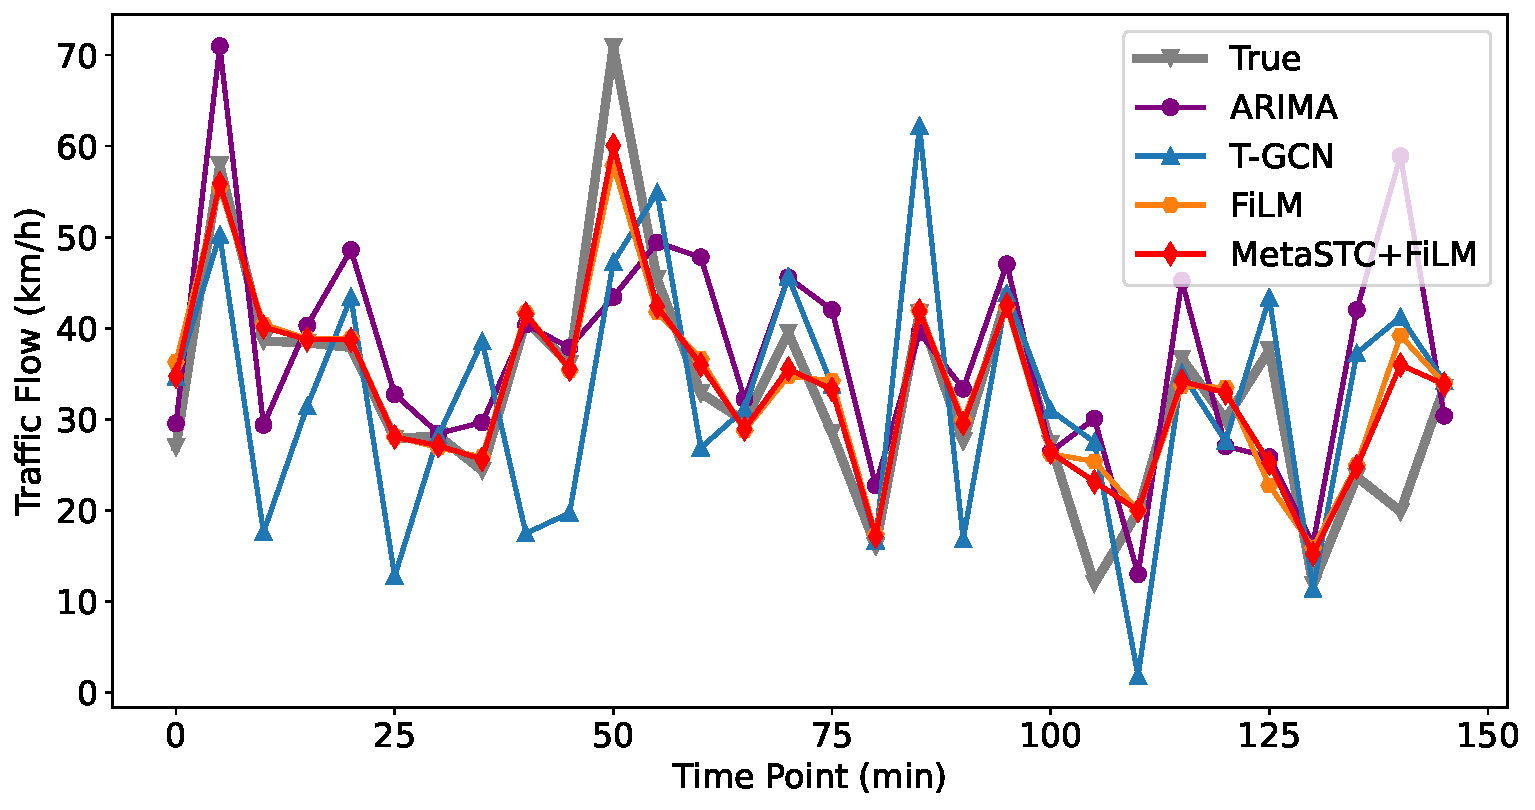
\includegraphics[width=8cm]{figure/MetaSTC_predict.pdf}
\caption{\textcolor{blue}{Prediction Curves}}
\label{fig:res}
\end{figure}


% These GCN-based methods were originally applied to traffic flow prediction for more than 200 roads, while our dataset contains nearly 8000 edges and the adjacency matrix is sparse, which makes it difficult for the GCN-based model to achieve good performance. 

% And although the ARIMA method is fast to train and has good performance on metrics such as MAE, it performs poorly on R$^2$, which indicates that the ARIMA method does not predict the future trend of traffic flow well. 

% To be mentioned, we attempted to utilize a GPU device with a VRAM of 24GB and a RAM of 80GB to train the AST-GNN model. However, due to the gross number of roads in our graph network, we experienced a memory overflow issue. This highlights the fact that GNN networks often require substantial computational resources, particularly when dealing with adjacency matrix operations that demand significant memory usage. Remarkably, our model does not exhibit such problems and demonstrates excellent performance in handling large-scale networks of this nature.

% The experimental results show that the STC-ML model achieves the best performance when combined with the advanced deep learning model FiLM and its training time is lower than the original FiLM model. 



% Our framework supports embedding different time-series prediction models. When embedding more complex models, the prediction accuracy may improve, but a more complex model requires longer time, it is no longer possible to iterate the model parameters quickly in combination with real-time data. Table~\ref{tab:TCN} shows the model performance and training time using LSTM and Temporal Convolutional Network (TCN) as time-series prediction components. The use of TCN optimizes the prediction accuracy by around 25\% but leads to a 20 times increase in training time. For specific application scenarios, we can combine the scenario requirements on prediction accuracy and training time to consider which temporal prediction model to use to embed in the STC-ML framework. Moreover, our framework can be extended to any traffic flow prediction model to accommodate different accuracy and arithmetic requirements, improving the efficiency and accuracy of the metamodel. 

% Additionally, as is shown in Fig xxx, our model is also more efficient in terms of time resources, requiring less computation time than the other models.  This might be because of the clustering module's ability to reduce the number of parameters required to learn the underlying patterns and to be convergence.

% In summary, the experimental results demonstrate the superior performance of our model in terms of both prediction accuracy and operational efficiency compared with statistic algorithms and state-of-the-art deep learning models.

\subsection{Ablation Study: RQ2}
In this section, we perform ablation studies to analyze the influence of key components within MetaSTC. The LSTM model is used to make the model lightweight and fast trainable. The experimental results are recorded in Figure~\ref{fig:abla}. We conducted a comparison between our complete MetaSTC model and two ablated versions to assess their respective performances. The first ablated version lacked the meta-learning component~(in yellow), while the second one did not incorporate the clustering module~(in green).

\begin{figure}
\centering
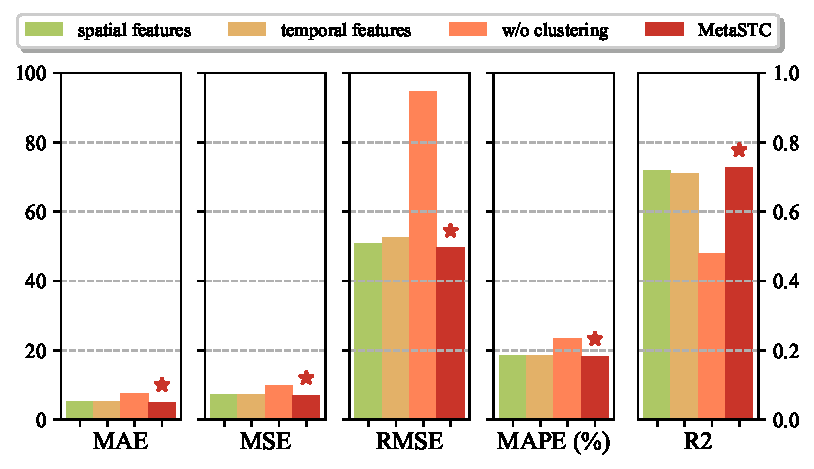
\includegraphics[width=8.5cm]{figure/ablation.pdf}
\caption{Prediction Accuracy of MetaSTC and Ablation Versions of Major Parts in the Model}
\label{fig:abla}
\end{figure}

 \begin{itemize}
     \item  Effect of Clustering Module: We observed that the clustering-based model outperformed the direct prediction model, with a 48.2\% reduction in MAE error. By partitioning the data into different clusters, the model can filter out outliers that do not belong to a particular category and focus on the features of a specific category, thus more accurately capturing the intrinsic patterns of the data in that category. In part~\ref{Q3} we further analyzed and interpreted the results of the clustering.
     \item Effect of Meta-Learning Module: The experiment results indicated that the inclusion of meta-learning had a significant positive impact on the model's performance, resulting in a 32.9\% reduction in MAE error compared to the ablated version. By accumulating experience on multiple tasks, meta-learner allows our model to perform better on unseen data. We also show in part~\ref{Q3} that the models that incorporate our framework converge faster (training time).
 \end{itemize}

\color{blue}

\subsection{Interpretability Analysis: RQ2}
\label{Q2}
To visualize the effectiveness of our clustering module, we randomly selected two clusters and then sampled 30 roads in each of them. As is depicted in the figure~\ref{fig:pearson}, the Pearson coefficients within clusters are neatly organized than between clusters (overall high or low). The Pearson coefficients of the road sequences within the first clusters are higher, which proves that they have more temporal similarity. The pearson coefficients within the second clusters are lower, which means that their similarity is mainly in spatial characteristics.
\begin{figure}[htbp]
\centering
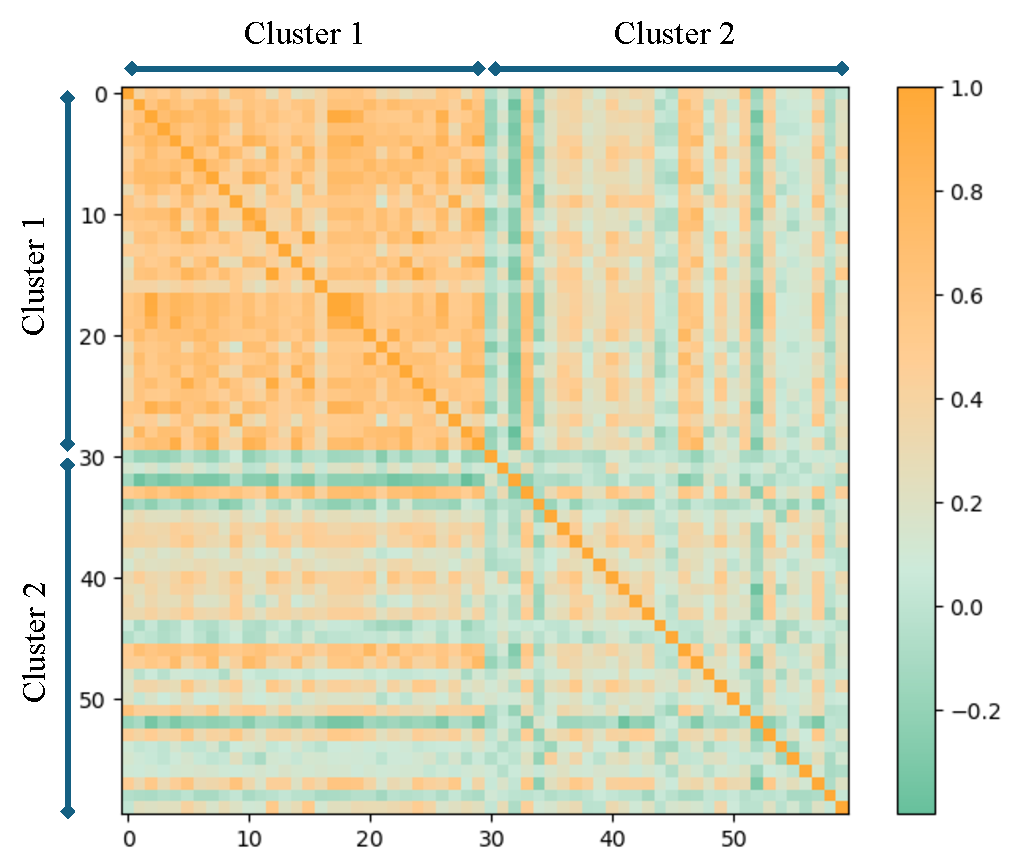
\includegraphics[width=6cm]{figure/Pearson.pdf}
\caption{\textcolor{blue}{Pearson Coefficients of Traffic FLow Sequences}}
\label{fig:pearson}
\end{figure}

In order to further analyze the results of clustering, we do the statistics of various spatial and temporal features of different clusters. The figure~\ref{fig:cluster} shows the distribution of temporal features (e.g. number of lanes shown in Figure~\ref{fig:cluster_temp}) and the spatial features (e.g. average traffic flow shown in Figure~\ref{fig:cluster_spat}) for our five obtained clusters. First, the intra-cluster features have similarities and the inter-cluster features have significant differences in distribution. This indicates that the clustering algorithm may be effective in grouping data points with similar attributes together. These clustering results have some degree of internal consistency. Models tend to cluster areas with similar roadway structures or designs. The similarity in average flows reveals that the model also does a good job of aggregating different traffic patterns.

At the same time, we note the tendency to aggregate lower lane count lane counts, such as the third cluster in the Figure~\ref{fig:cluster}, which also aggregates to lane couples with lower average flows. This may indicate that there is some match between roadway design (fewer lanes) and traffic demand (lower flows) in certain areas. Fewer lanes may be sufficient to meet traffic flow demands in these areas. This is in line with our usual perceptions and also shows that there will be some correlation between spatial and temporal features.

\color{black}


\begin{figure}[htbp]
\centering
\begin{minipage}[t]{0.24\textwidth}
\centering
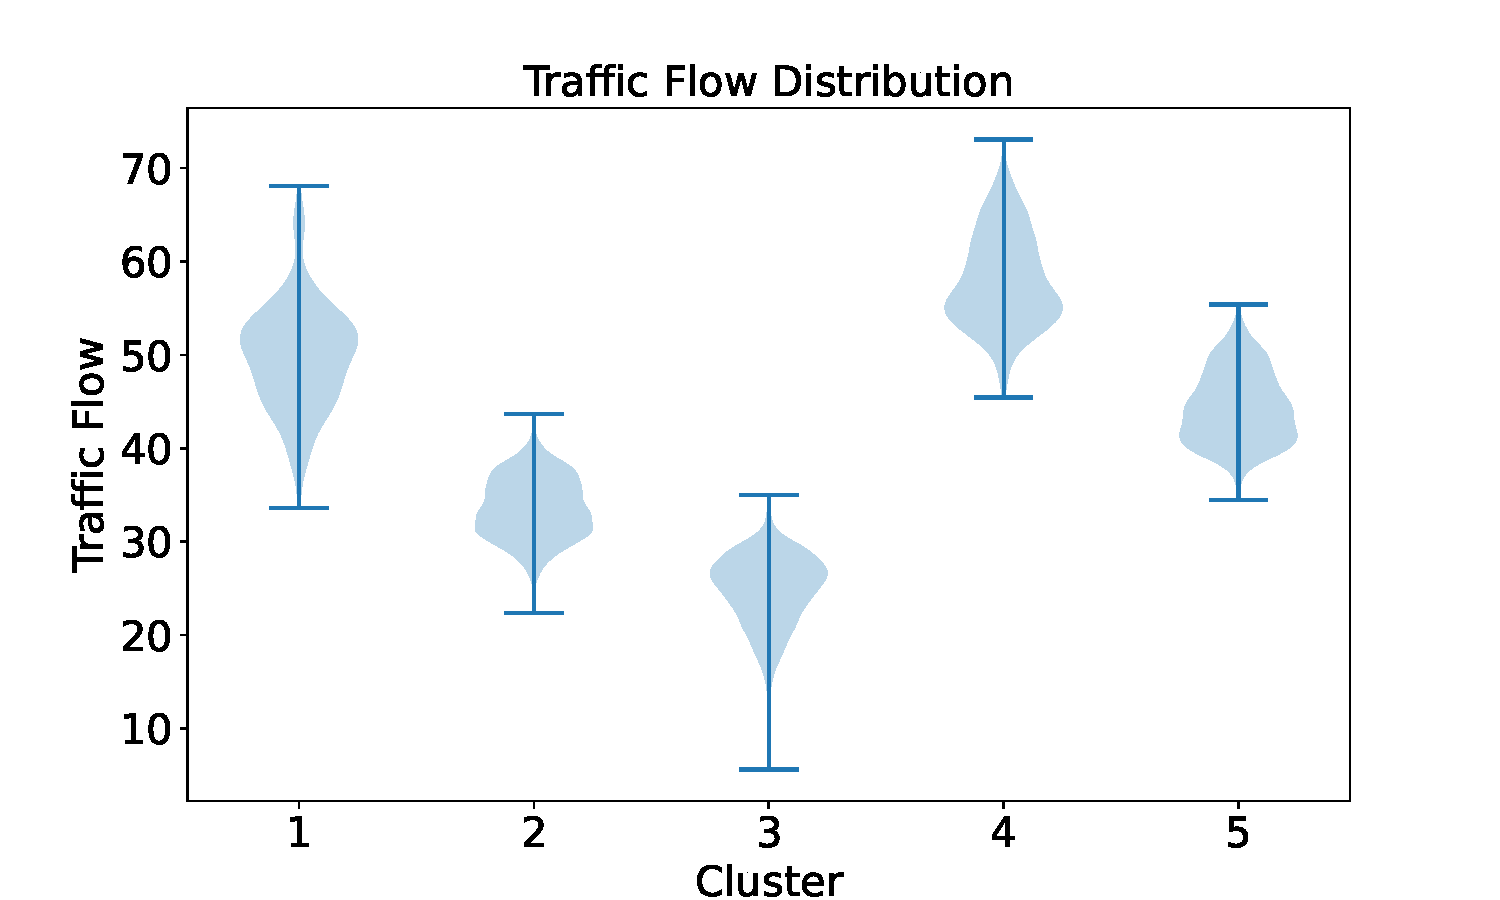
\includegraphics[width=4.5cm]{figure/cluster_traffic.pdf}
\subcaption{Traffic Flow}
\label{fig:cluster_temp}
\end{minipage}
\begin{minipage}[t]{0.24\textwidth}
\centering
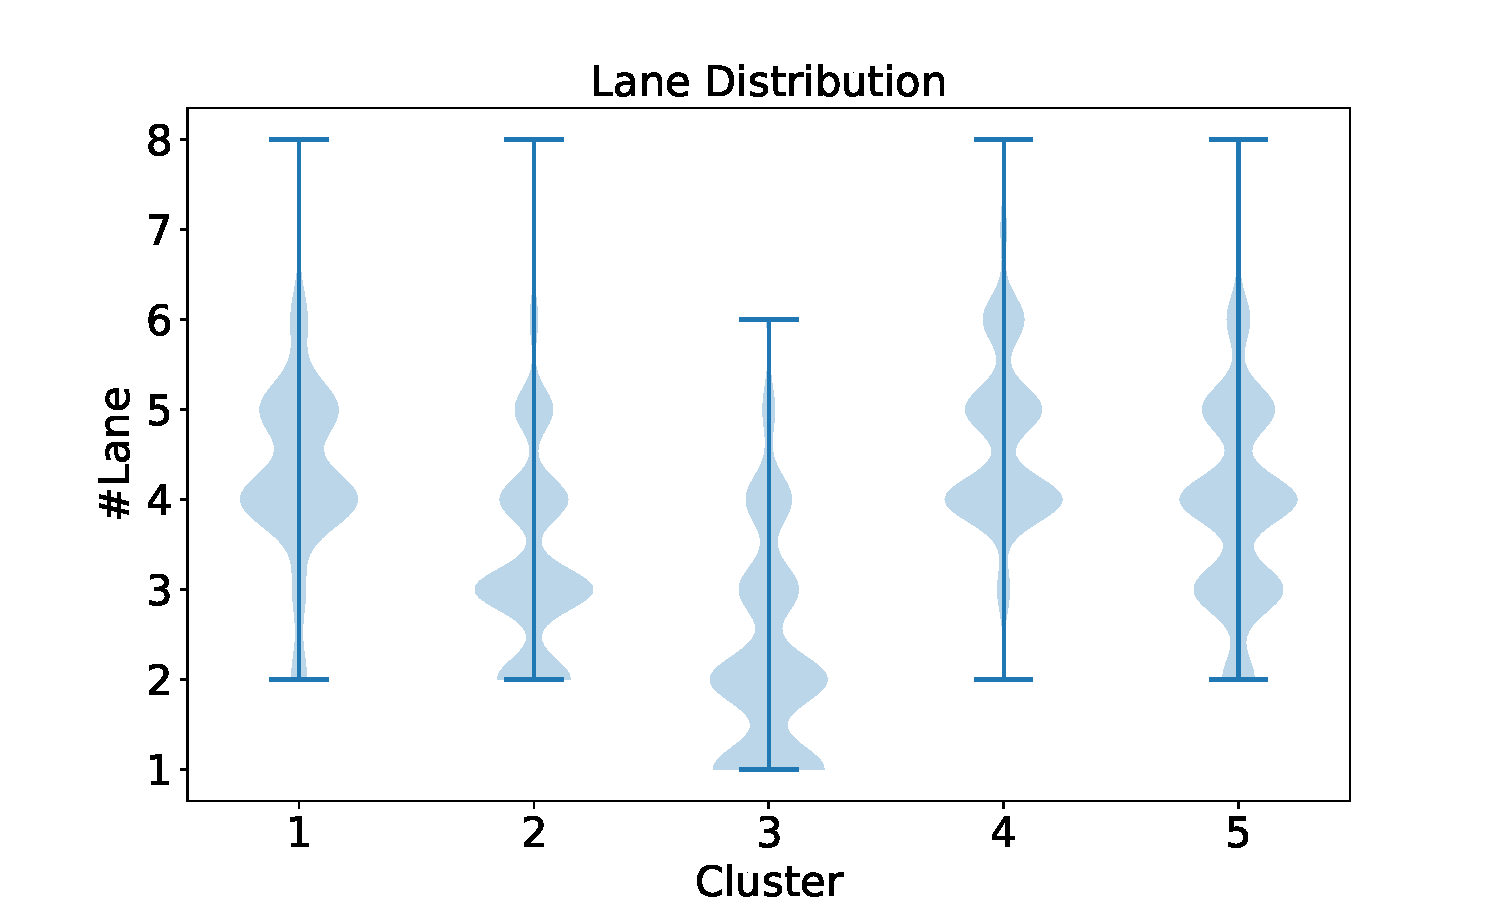
\includegraphics[width=4.5cm]{figure/cluster_lane.pdf}
\subcaption{Number of Lanes}
\label{fig:cluster_spat}
\end{minipage}
\caption{\textcolor{blue}{Clustering Results}}
\label{fig:cluster}
\end{figure}

\subsection{Comparative Results: RQ3}
\label{Q3}
To show the effectiveness of our models in lightweight time series prediction models, we use the monetary cost of renting training GPUs and the time cost consumption as a measure. We use the GPU rental cost of 0.4 dollars per hour as a standard to estimate the training budget overhead of 500,000 roads per city. The cost consumption comparison of different models is shown in Table \ref{tab:cost}. 

\begin{table}[htbp]
    \centering
    \caption{Hourly Cost Estimation With and Without MetaSTC per City.}
  \label{tab:cost}
  \setlength{\tabcolsep}{2mm}
  \resizebox{0.5\textwidth}{!}{%
    \begin{tabular}{lcccc}
    \toprule  
    Model & Beijing & Shanghai & California \\
  \midrule
    LSTM & 3.59 & 3.24 & 2.26 \\
    MetaSTC+LSTM & 1.90~(47.0\%$\downarrow$) & 0.25~(92.3\%$\downarrow$) & 0.19~(91.7\%$\downarrow$) \\
    FiLM & 20.35 & 21.83 & 13.58 \\
    MetaSTC+FiLM & 14.66~(30.0\%$\downarrow$) & 2.24~(89.7\%$\downarrow$) & 1.59~(88.2\%$\downarrow$)\\
    % \midrule
    %   TCN & & & \\
    % MetaSTC+TCN & & & \\
    % \midrule
    %   FiLM & & & \\
    % MetaSTC+FiLM & & & \\
    \bottomrule  
    \end{tabular}}
\end{table}

\color{blue}

Besides, in scenarios where efficiency is more emphasized, we can combine the MetaSTC model with a more concise deep learning model such as LSTM to achieve a shorter training time. This demonstrates the advantages of MetaSTC in real-world applications. We can consider which prediction model to combine the MetaSTC model with in conjunction with the scenario's requirements on accuracy and cost.

\subsection{Parameter Study: RQ3}

\begin{figure}[htbp]
\centering
\begin{minipage}[t]{0.24\textwidth}
\centering
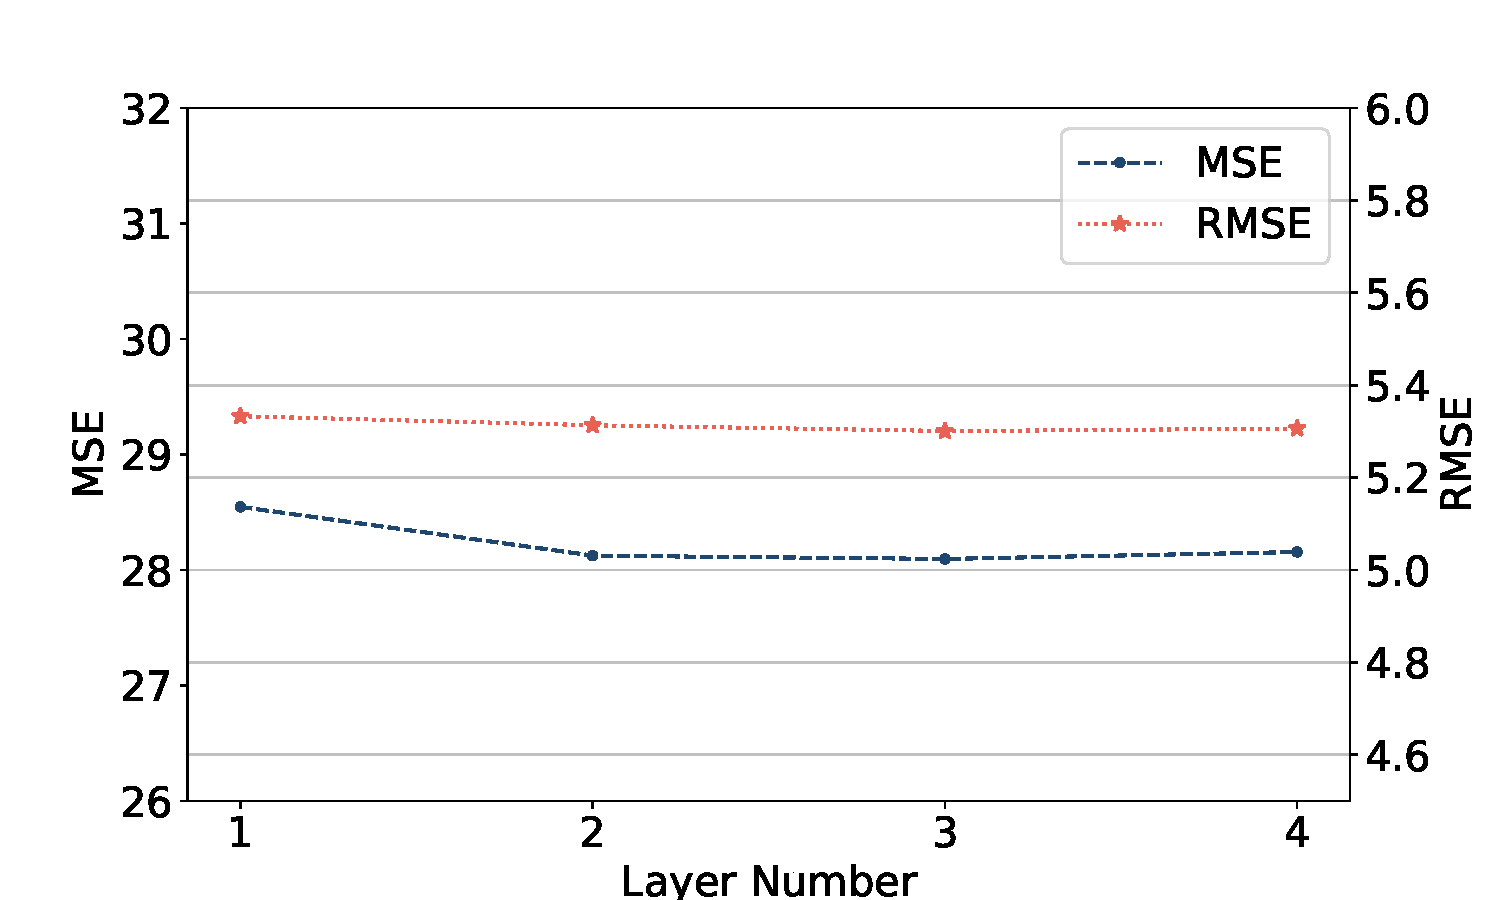
\includegraphics[width=4.5cm]{figure/layer.pdf}
\subcaption{Layer Number}
\label{fig:layer}
\end{minipage}
\begin{minipage}[t]{0.24\textwidth}
\centering
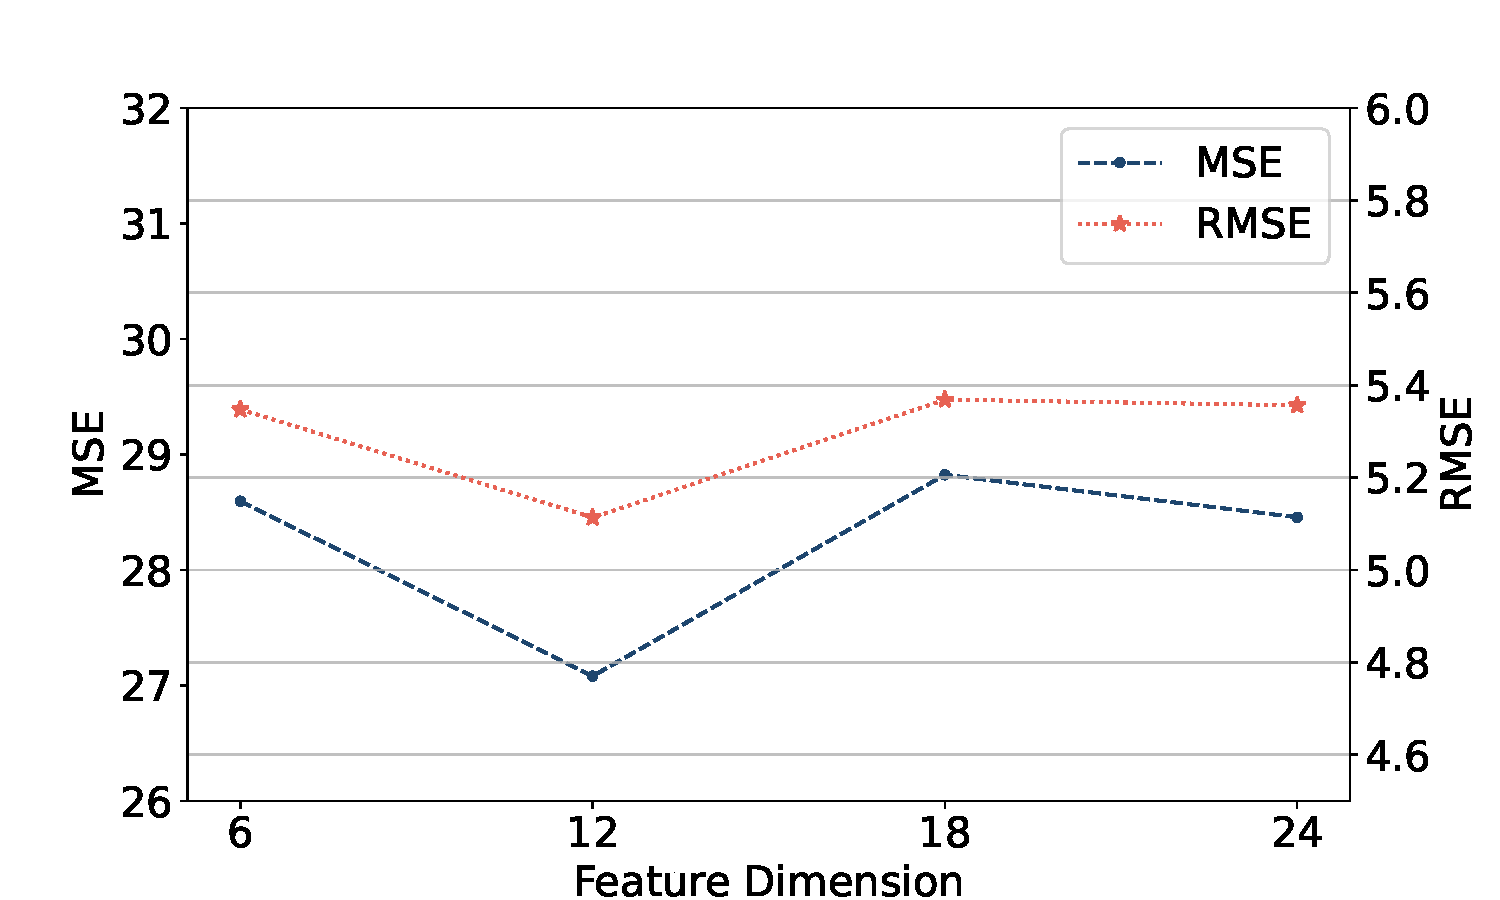
\includegraphics[width=4.5cm]{figure/feature_dimension.pdf}
\subcaption{Feature Dimension}
\label{fig:feature}
\end{minipage}
\begin{minipage}[t]{0.24\textwidth}
\centering
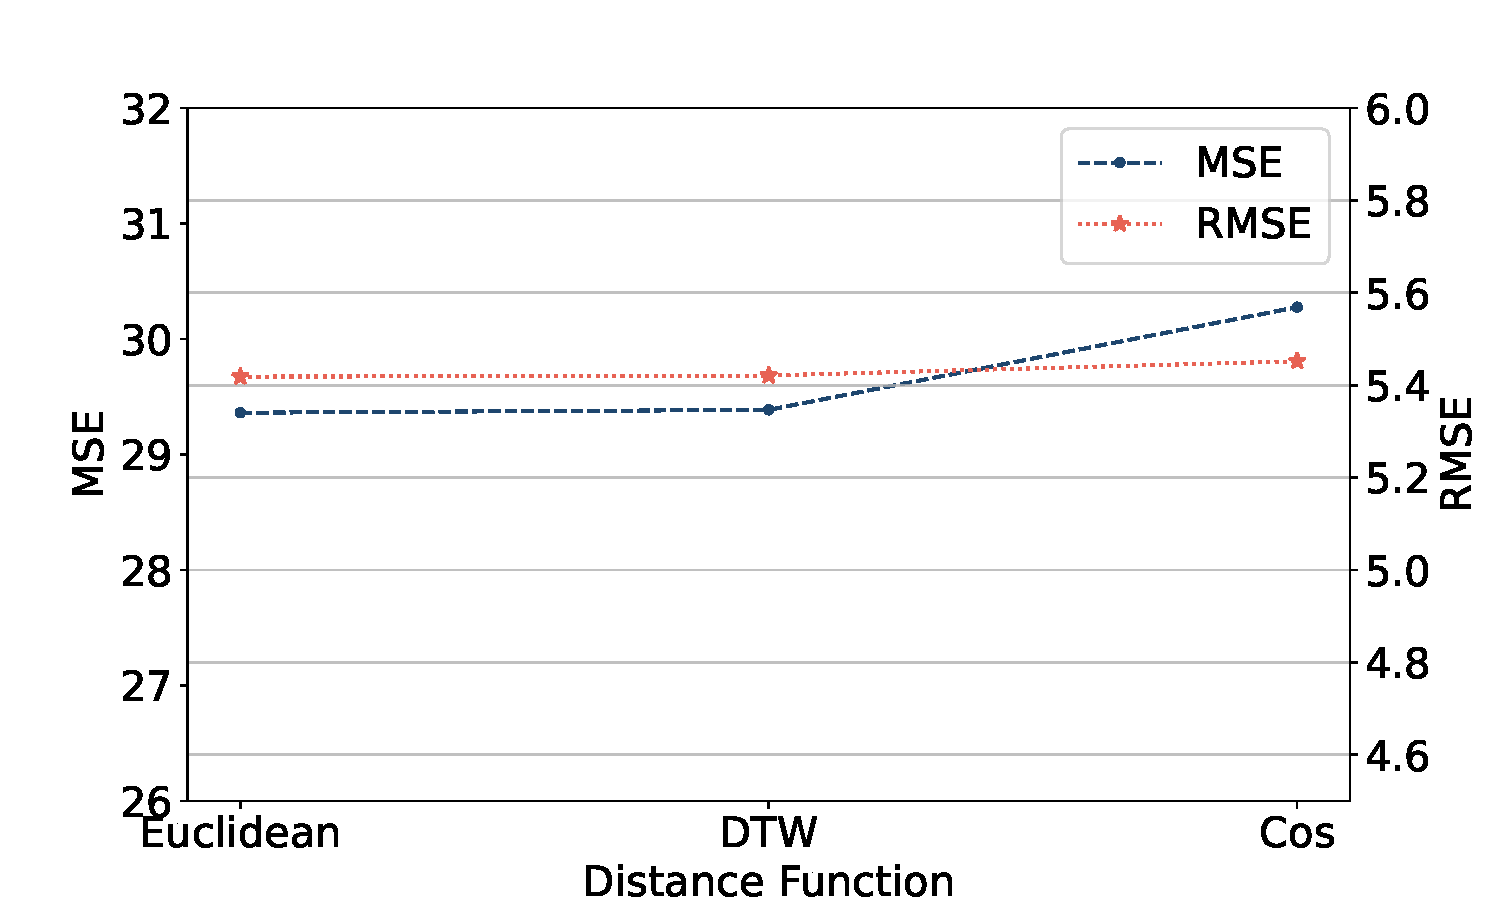
\includegraphics[width=4.5cm]{figure/dis.pdf}
\subcaption{Distance Function}
\label{fig:dis}
\end{minipage}
\begin{minipage}[t]{0.24\textwidth}
\centering
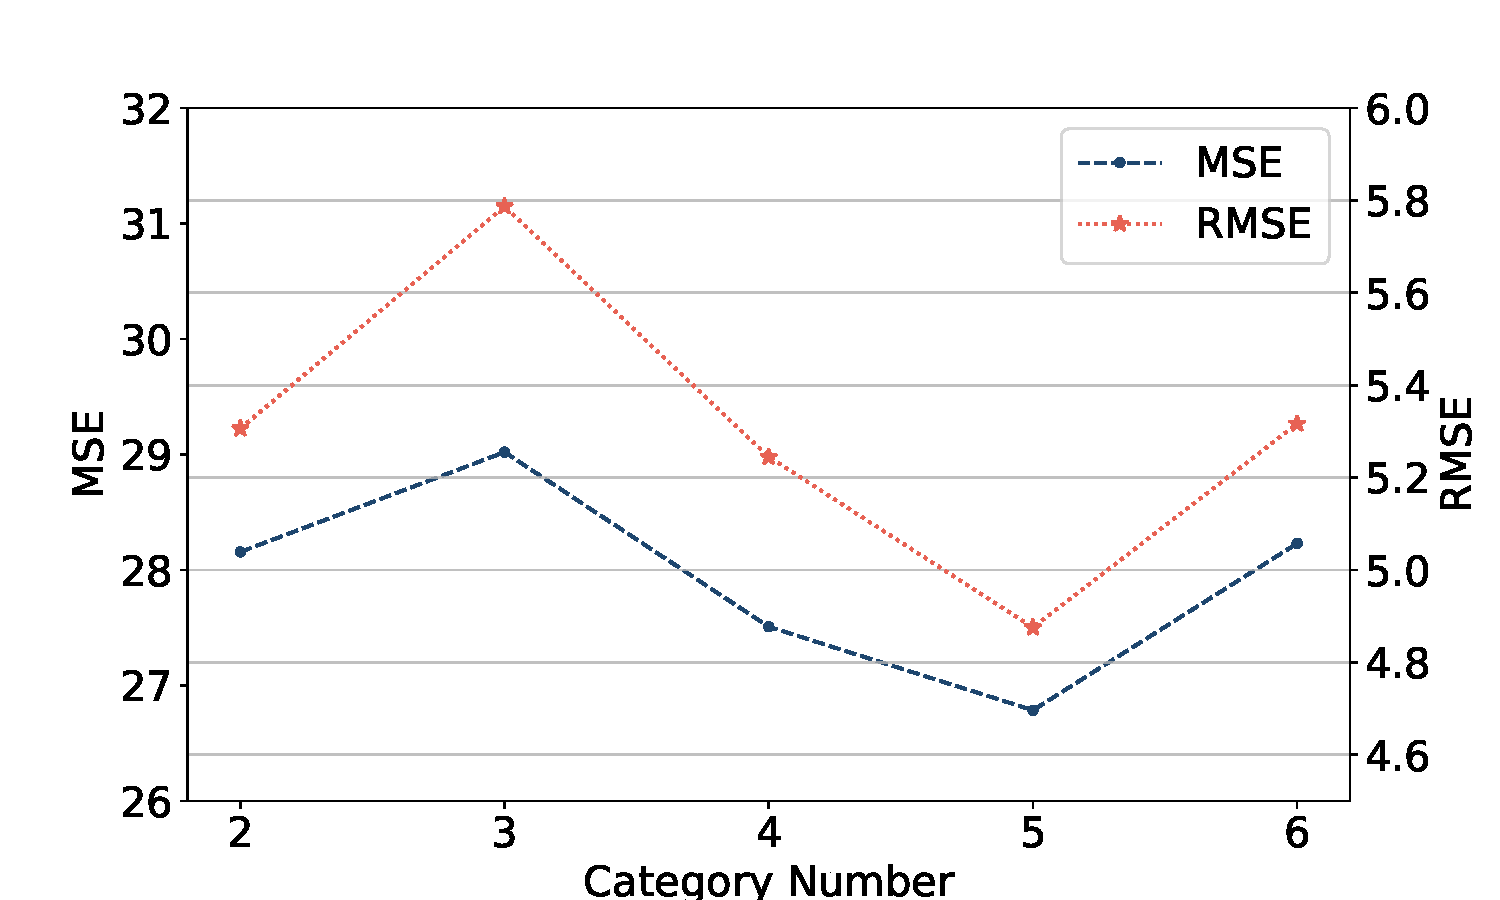
\includegraphics[width=4.5cm]{figure/category.pdf}
\subcaption{Category Number}
\label{fig:category}
\end{minipage}
\caption{Parameter Study.}
\label{fig:parameter}
\end{figure}

We test the effect of the dimensionality reduction of temporal features, clustering distance functions, clustering categories, and the number of layers in the prediction meta-learner. We tried different parameter settings as is shown in Figure~\ref{fig:parameter}. The choice of the number of layers and the choice of the distance equation have a marginal effect on the result, however, the choice of the dimensionality of the features and the number of clusters have a significant effect on the accuracy.

\section{Discussion}
\subsection{Application Potential and Practical Implications}

Beyond addressing technical challenges, MetaSTC offers substantial potential for real-world traffic management. One key application lies in congestion prediction and mitigation. For example, our clustering module (Fig. 9) identifies distinct traffic patterns, such as Cluster 1 with high average flows during peak hours, indicative of urban bottlenecks (e.g., business districts in Beijing). By integrating MetaSTC’s predictions, traffic authorities could dynamically adjust signal timings—extending green phases for high-flow clusters during rush hours—reducing delays based on baseline flow reductions observed in our LargeST dataset (Table IV). This targeted optimization leverages the model’s ability to isolate critical zones, enhancing urban mobility without requiring extensive infrastructure upgrades. 

% Another promising application is cross-city model transferability, addressing Challenge 3’s spatio-temporal diversity. The backbone-agnostic design allows MetaSTC to adapt pre-trained parameters from one city (e.g., Beijing, with 7949 roads) to another (e.g., Shanghai, with 5144 roads) by fine-tuning on local data. Experiments on PeMS04 and LargeST datasets suggest that fine-tuning with as little as 20\% of a new city’s data achieves MAE reductions comparable to full retraining (Table IV), thanks to the meta-learner’s task-shared priors. This transferability could significantly lower deployment costs for municipalities with limited data resources, fostering scalable traffic solutions across heterogeneous urban landscapes.

Real-time applicability is equally critical, as traffic systems often demand instantaneous forecasting. MetaSTC’s lightweight design, evidenced by reduced training times (Table V), supports online learning scenarios. Algorithm 1, which rapidly encodes new roads into clusters via spatio-temporal embeddings, enables incremental updates without retraining the entire model. For instance, adding a newly monitored road in Shanghai could be processed in seconds by assigning it to an existing cluster and refining local parameters, maintaining prediction accuracy under dynamic conditions. This capability positions MetaSTC as a viable tool for adaptive traffic control systems, such as real-time rerouting during unexpected events like accidents or road closures.

\subsection{Future Directions}
Looking ahead, several avenues exist to enhance MetaSTC’s capabilities. One improvement could involve integrating Graph Neural Networks (GNNs) to strengthen spatial dependency modeling. While our current spatial embeddings (Table II) capture static attributes like road level and lane count, GNNs could dynamically model inter-road relationships (e.g., traffic spillovers between adjacent segments), potentially improving prediction accuracy on sparse networks like LargeST, where T-GCN underperformed (Table IV). This hybrid approach would complement the clustering module by refining subtask boundaries, though it may increase computational overhead, necessitating further efficiency optimizations. Alternatively, incorporating attention mechanisms into the spatio-temporal gating unit could enhance feature extraction. By assigning learnable weights to temporal cycles (e.g., daily vs. weekly) or spatial features (e.g., proximity vs. road hierarchy), the model could better prioritize dominant patterns, potentially reducing MAE by an additional 5-10\% based on trends in attention-based baselines like TimesNet (Table IV).

Another promising direction is multi-domain integration to bolster MetaSTC’s robustness. Traffic flow is influenced by external factors such as weather conditions or special events (e.g., holidays, accidents), which our current framework does not explicitly model. Extending the spatio-temporal representation (Eq. 1-2) to include weather data (e.g., precipitation intensity) or event indicators (e.g., binary flags for incidents) could improve prediction reliability, especially in volatile scenarios. For instance, coupling rainfall data with Cluster 3’s low-flow roads (Fig. 9) might reveal weather-induced slowdowns, enabling proactive traffic adjustments. Preliminary studies suggest that such integrations could reduce RMSE by up to 15\% in adverse conditions, aligning MetaSTC with comprehensive smart city systems. These enhancements would require expanded datasets and validation, offering a rich field for future exploration.

\color{black}

\section{Related Works}

\textbf{Traffic Flow Prediction}
In the early days of traffic flow prediction research, researchers usually used traditional statistical methods for time-series prediction, such as ARIMA~\cite{arima}. After that deep learning models were adopted as the amount of data increased. Convolutional Neural Networks~(CNN) have given rise to several excellent network models~\cite{DBLP:conf/iclr/WuHLZ0L23}. Besides, transformer~\cite{DBLP:conf/nips/VaswaniSPUJGKP17} and its variants~\cite{nips/LiJXZCWY19}~\cite{DBLP:conf/pkdd/FanYCWZWDZZ23}~\cite{DBLP:conf/aaai/JiangHZW23} are able to automatically learn and focus on the important parts of the input sequence for better understanding and processing of the sequence data through the attention mechanism. 

With the rise of Graph Neural Network~(GNN), there are a lot of GNN-based methods. They generally combine GNNs with either Recurrent Neural Networks (RNNs) or Temporal Convolutional Networks (TCNs) to capture intricate spatial and temporal dependencies in traffic data. ST-MetaNet~\cite{pan_urban_2019} and AGCRN~\cite{10.5555/3495724.3497218} employ RNNs and their variants. \textcolor{blue}{ASTCN~\cite{DBLP:conf/icdm/Zhang0SG021}, STGCN~\cite{stgcn} and GWN~\cite{graphwave} use dilated causal convolution for temporal patterns modeling. These approaches have exhibited promising performance on small-scale datasets, which, however, have limited size in terms of the number of nodes, edges, and time frames. This raises valid concerns about their scalability when applied to large-scale traffic forecasting datasets, which strive to encompass more realistic real-world scenarios.}

\textbf{Clustering in Traffic Flow Analysis}
Clustering algorithms have been widely used in the field of traffic flow analysis to improve the efficiency of traffic prediction problems. Clustering methods were first employed by Kuo et al. to improve traffic prediction~\cite{kuo_adaptive_2001}. After that, Tsai et al. developed a dual-module architecture comprising a Temporal Neighborhood Clustering module and an Incremental Learning module~\cite{tsai_incremental_2022}. Luo et al. demonstrated that clustering could be a promising solution to the smoothing problem of GCN networks~\cite{luo_clusterst_2023}.

However, these methods often rely on a single feature of traffic flow data while neglecting the intersectionality between different features. In contrast to these studies, our clustering method focuses on the interaction between spatial and temporal features and designs a gating mechanism for extracting the spatio-temporal features so that we can cluster together roads with similar patterns to avoid unevenness in prediction accuracy among roads.

\textbf{Meta-Learning in Traffic Flow Prediction}
Meta-learning is a machine-learning technique that aims to enable models to initialize parameters from the retrained models and adapt quickly to new environments or tasks. In recent years, meta-learning has become increasingly prevalent in predicting traffic flows. One widely used method involves extracting spatial information to initialize the parameters of the meta-model. Zhang et al. proposed an efficient meta-learning way that tunes the global model with specific heterogeneous information from different regions\cite{zhang_efficient_2022}. Besides, other features have also been used for meta-learning. For instance, Pan et al. incorporate two meta-learners to assist the predictions of the main model~\cite{pan_urban_2019}. Fang et al. fused two meta-learning modules that integrate temporal and spatial data dimensions~\cite{fang_meta-msnet_2021}. In addition, Wang et al. conducted a study on graph structure in meta-learning~\cite{wang_deep_2022}. Our model first combines clustering results and meta-learning techniques in traffic flow prediction. We also designed a meta-learning method to incorporate context information into the meta-learning model.

\section{Conclusion}

Traffic flow prediction is one of the most important tasks for providing convenient and efficient urban transportation services. In this paper, we analyze the shortcomings of previous methods that fail to achieve the result as well as the original on large-scale datasets in prediction accuracy and operational efficiency. We propose a backbone agnostic spatio-temporal framework based on clustering and meta-learning named MetaSTC, which is capable of fast training and improving prediction accuracy. We conduct experiments on real-world datasets that contain thousands of roads and show that our model outperforms SOTA baselines. We conduct ablation experiments to demonstrate the importance of the clustering module and the meta-learning module, which can provide huge performance improvements. Our paradigm provides an effective and robust interface for accelerating and lightweight time-series prediction models.

\section{Acknowledgements}

We are deeply grateful to all who have contributed to this paper. Special thanks go to Kexin Xu and Zhemeng Yu. Kexin Xu provided research thinking with profound expertise. Zhemeng Yu dedicated great efforts to data collection and analysis, laying a solid foundation for the empirical part of the paper.

This work was supported by the National Key R\&D Program of China [2024YFF0617700], the National Natural Science Foundation of China [U23A20309, 62272302, 62372296], and the CCF-DiDi GAIA Collaborative Research Funds for Young Scholars [202404].


\bibliographystyle{splncs04}
\bibliography{traffic-prediction}

\begin{IEEEbiography}[{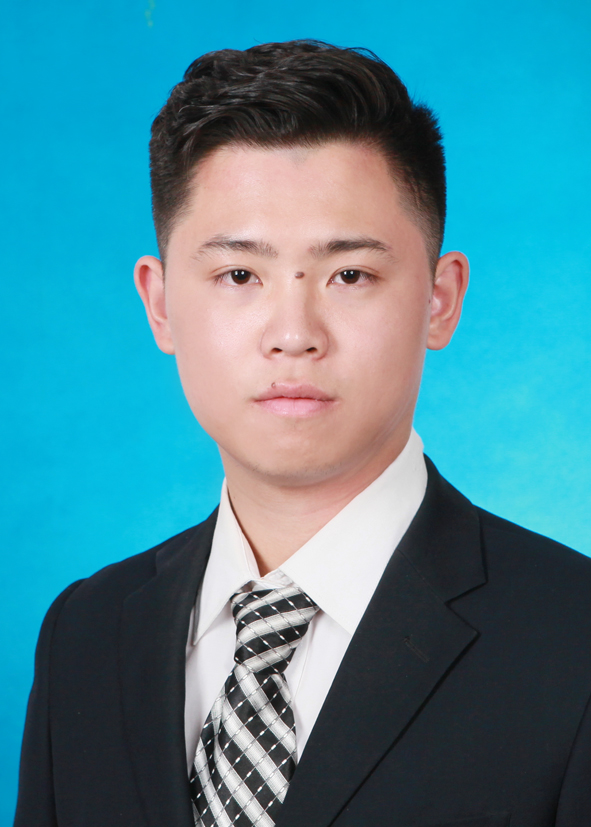
\includegraphics[width=1in,height=1.25in,clip,keepaspectratio]{figure/yucengao-2.jpg}}]{Yucen Gao} 
received the B.S. and Ph.D. degree from Shanghai Jiao Tong University, China, in 2020 and 2025. He is currently an associate professor with the Software College of Northeastern University. His research interests data engineering and network optimization. He has published more than 20 papers in high-ranked international conferences and journals such as TMC, TON, SIGKDD, SIGIR, ICDE, WWW, etc.
\end{IEEEbiography}

\begin{IEEEbiography}[{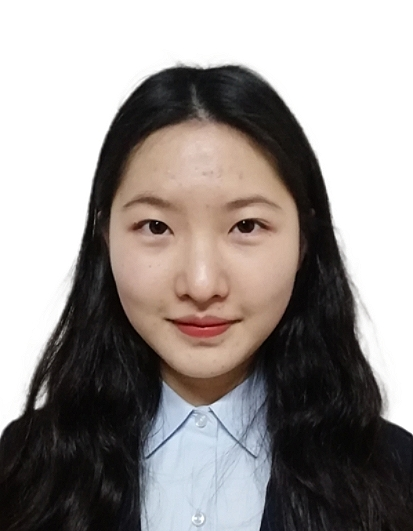
\includegraphics[width=1in,height=1.25in,clip,keepaspectratio]{figure/Huang_Guorun.jpg}}]{Guorun Huang}
received the B.S. degree from Shanghai Jiao Tong University, China, in 2022. She is currently a graduate student in the Khoury College of Computer Science at Northeastern University, USA. Her research interests lie in optimal algorithms, machine learning and computer vision. She has published two papers in Journal of Analytical and Applied Pyrolysis and Renewable Energy.
\end{IEEEbiography}

\begin{IEEEbiography}
[{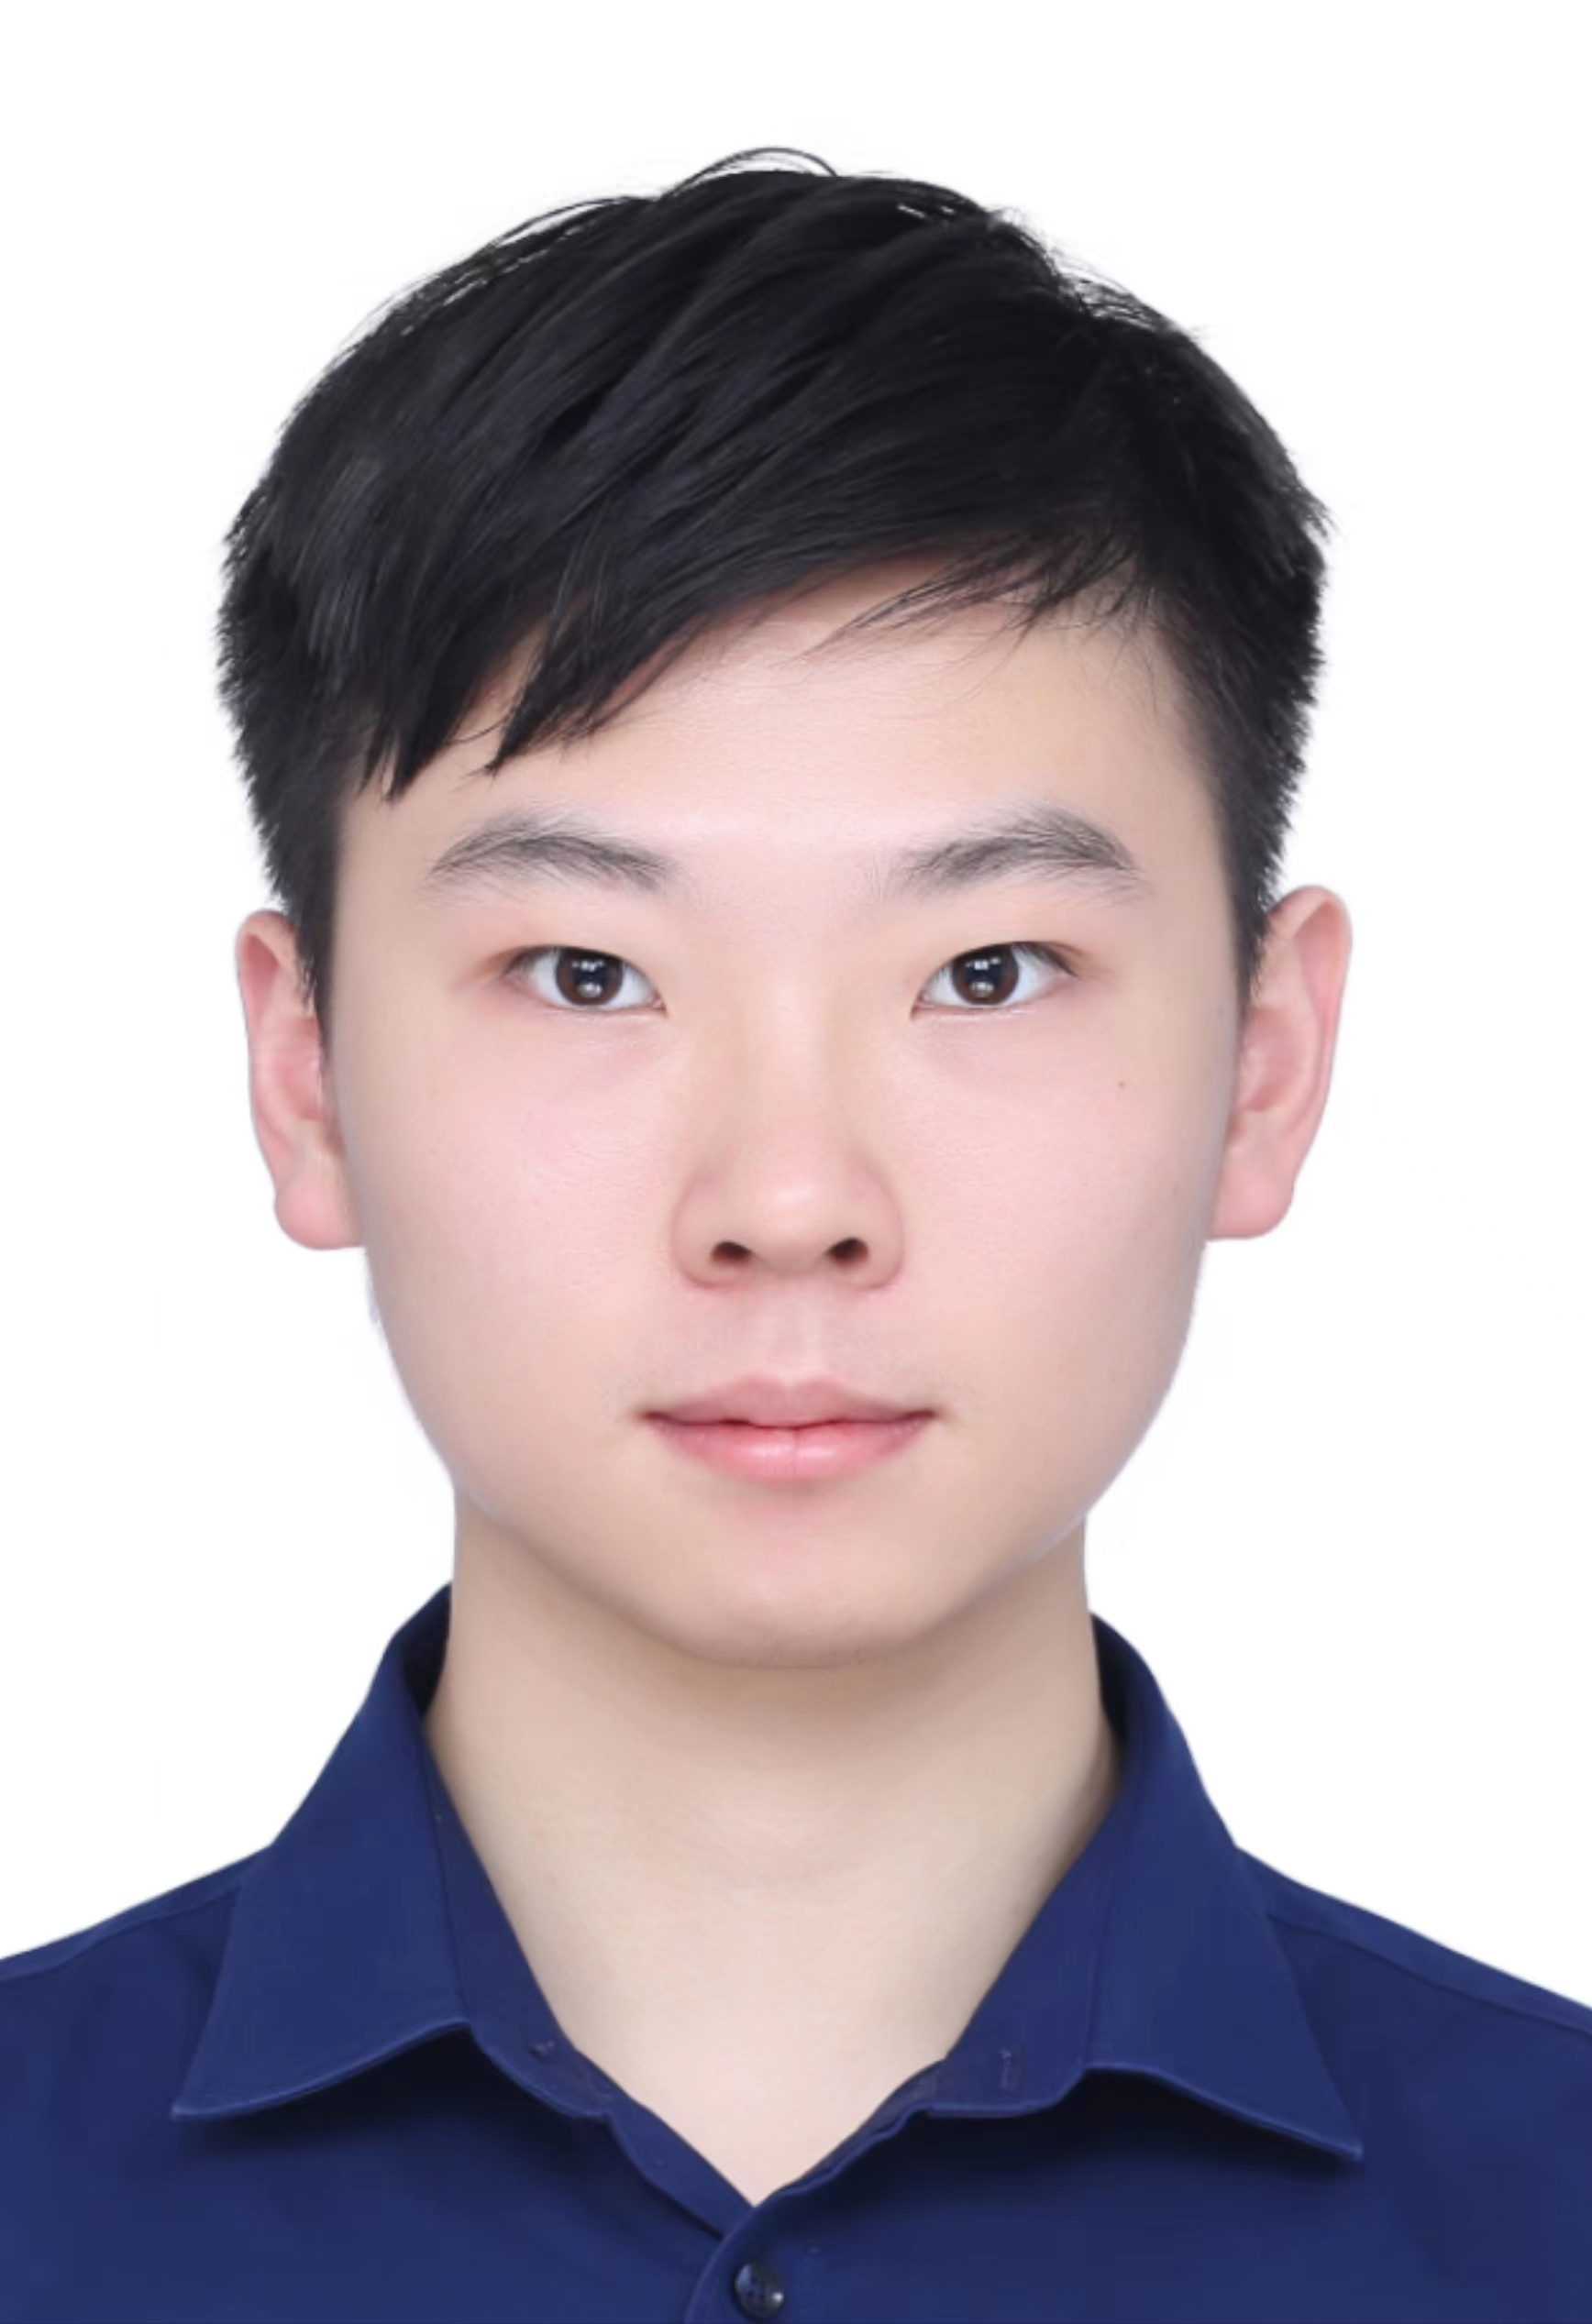
\includegraphics[width=1in,height=1.25in,clip,keepaspectratio]{figure/picture.jpg}}]{Bokai Lin}
received the B.S. degree from Shanghai Jiao Tong University, China. He is currently pursuing the Ph.D. degree jointly with Shanghai Jiao Tong University and Shanghai Innovation Institute.
His research interests include large language models, generative agents, recommender systems, and intelligent robotics. 
He has co-authored papers in top machine learning conferences and journals, including ICLR, ICML, and NeurIPS.
\end{IEEEbiography}

% \begin{IEEEbiography}[{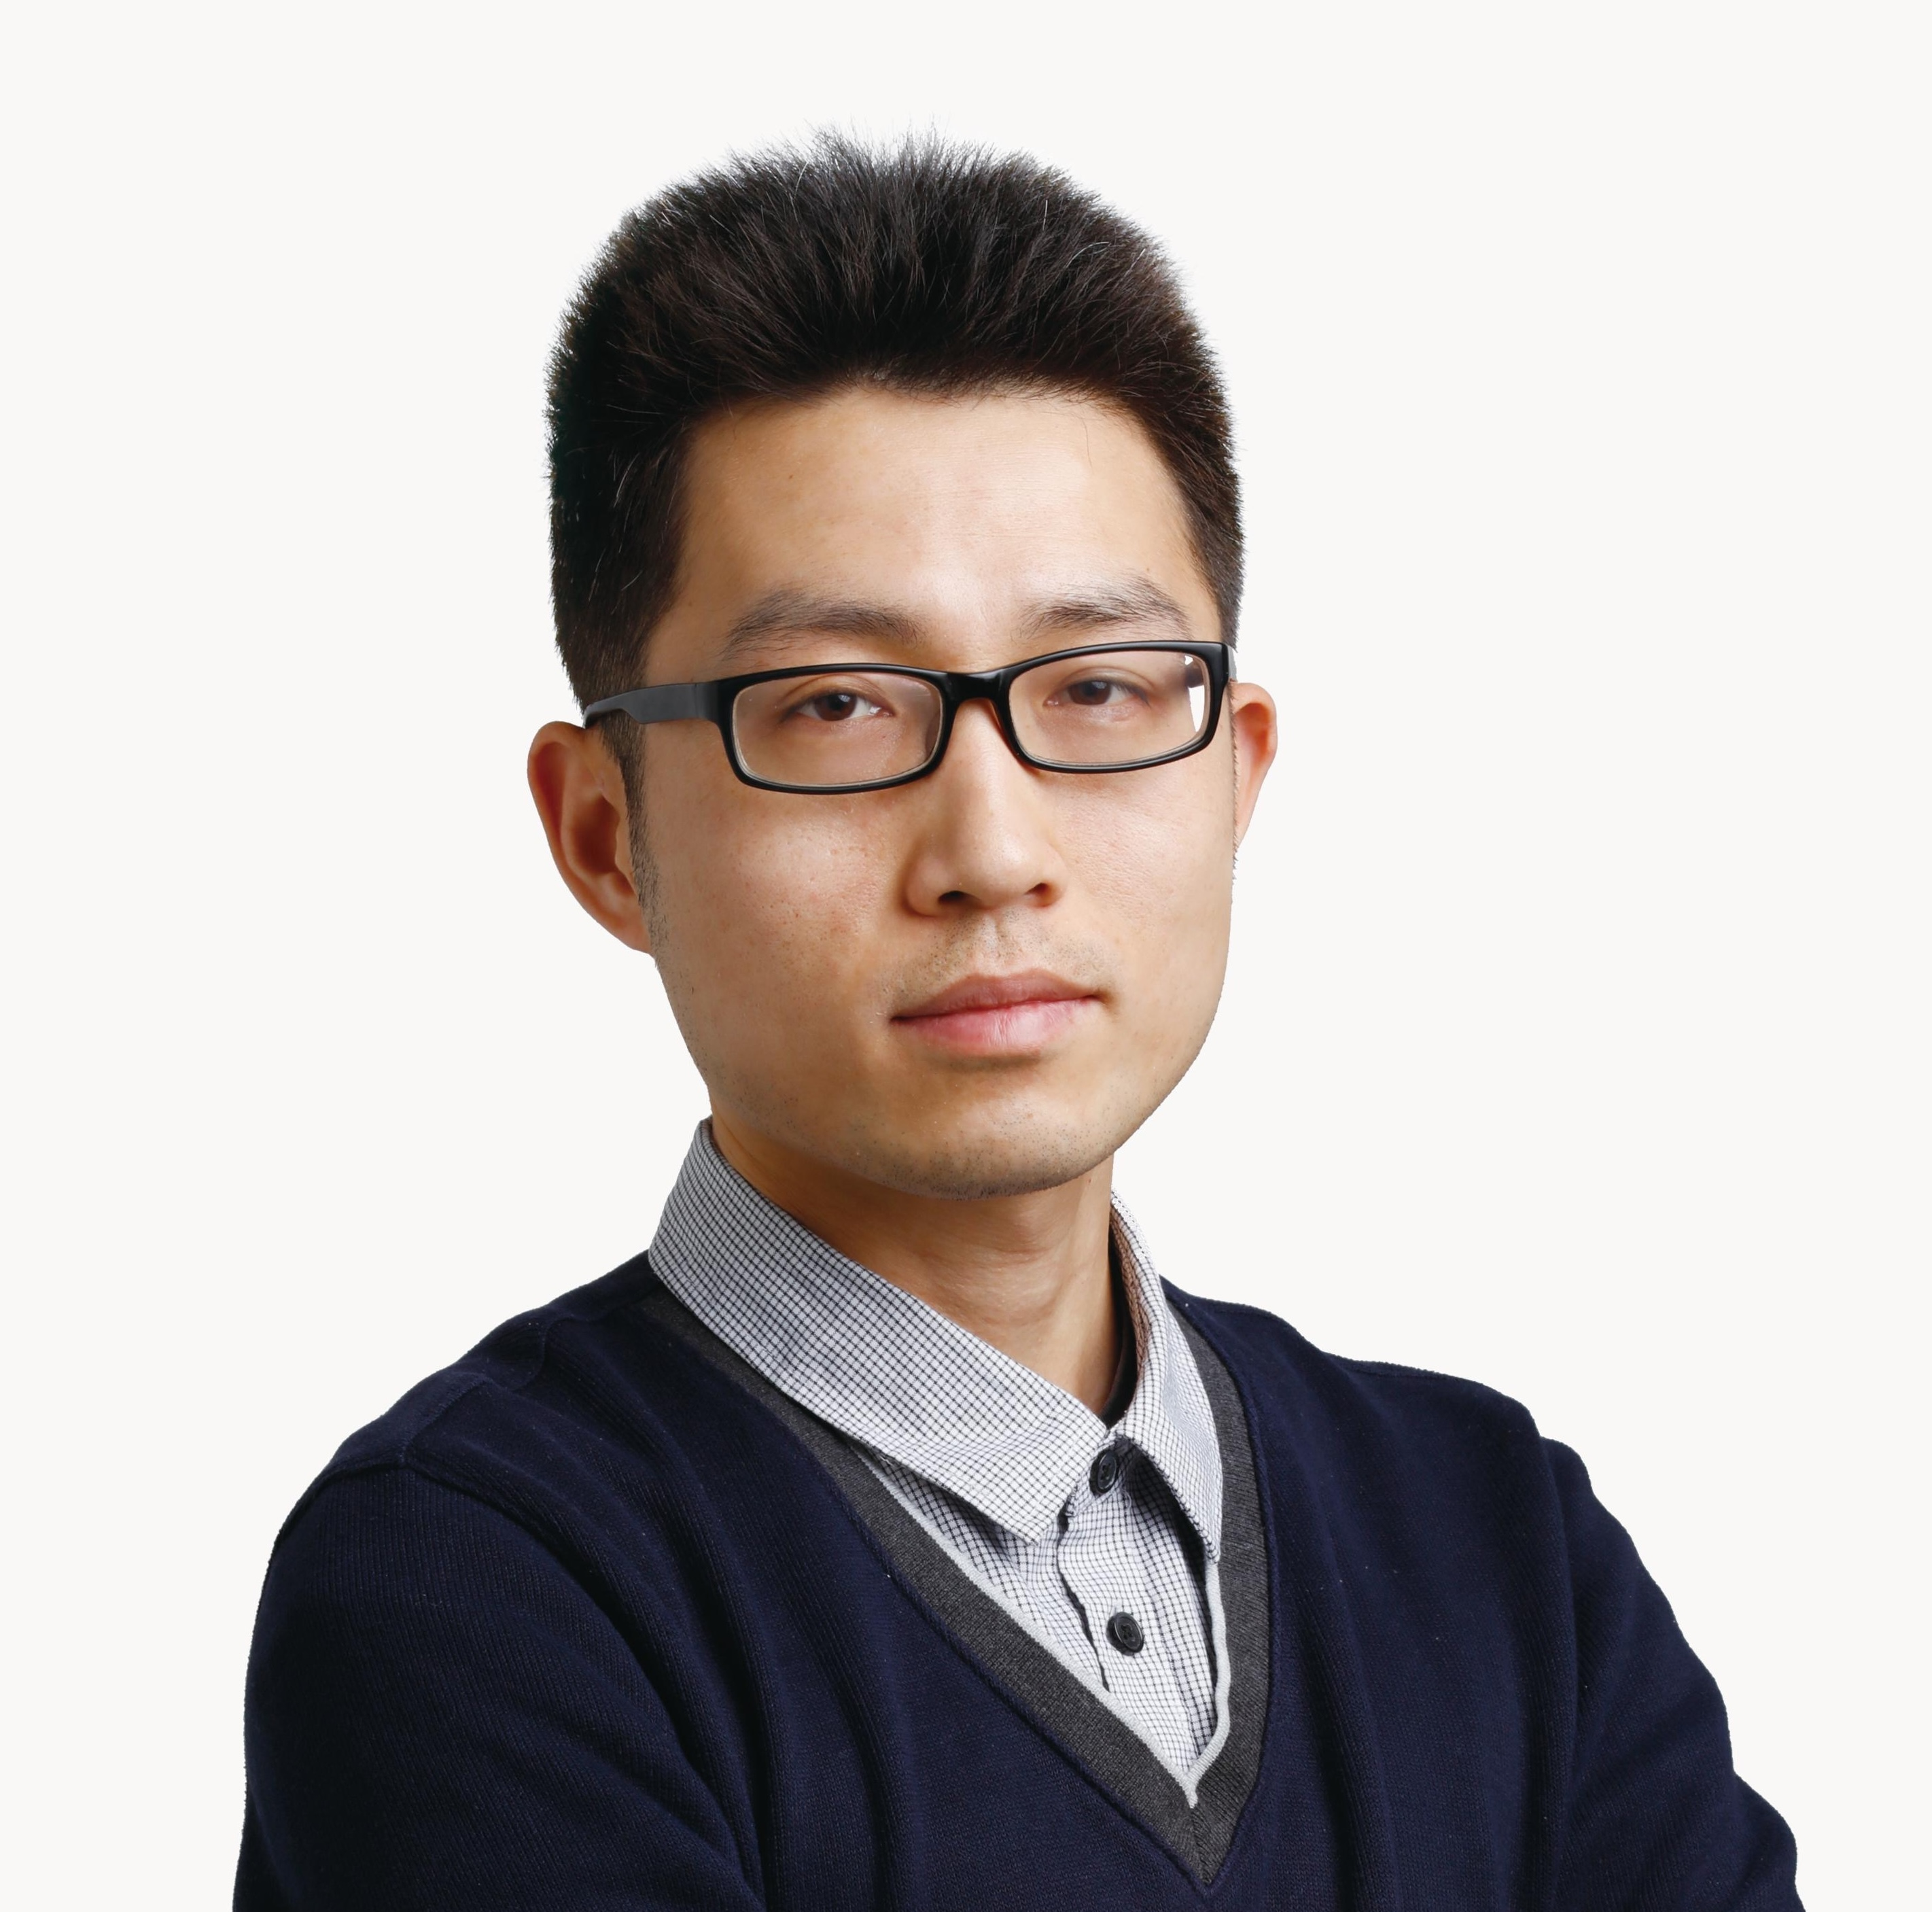
\includegraphics[width=1in,height=1.25in,clip,keepaspectratio]{figure/JunFang-2.jpg}}]{Jun Fang} 
% received the B.S. degree from the Hefei University of Technology, China, in 2009, and the M.S. degree from the University of Science and Technology of China, China, in 2012. He is currently the Chief Algorithm Engineer with the Maps and Public Transportation Department, DiDi Company, Beijing, China, and in charge of estimated time of arrival and route planning. His research interests include machine learning, deep learning, and spatio-temporal forecasting.
% \end{IEEEbiography}

\begin{IEEEbiography}
[{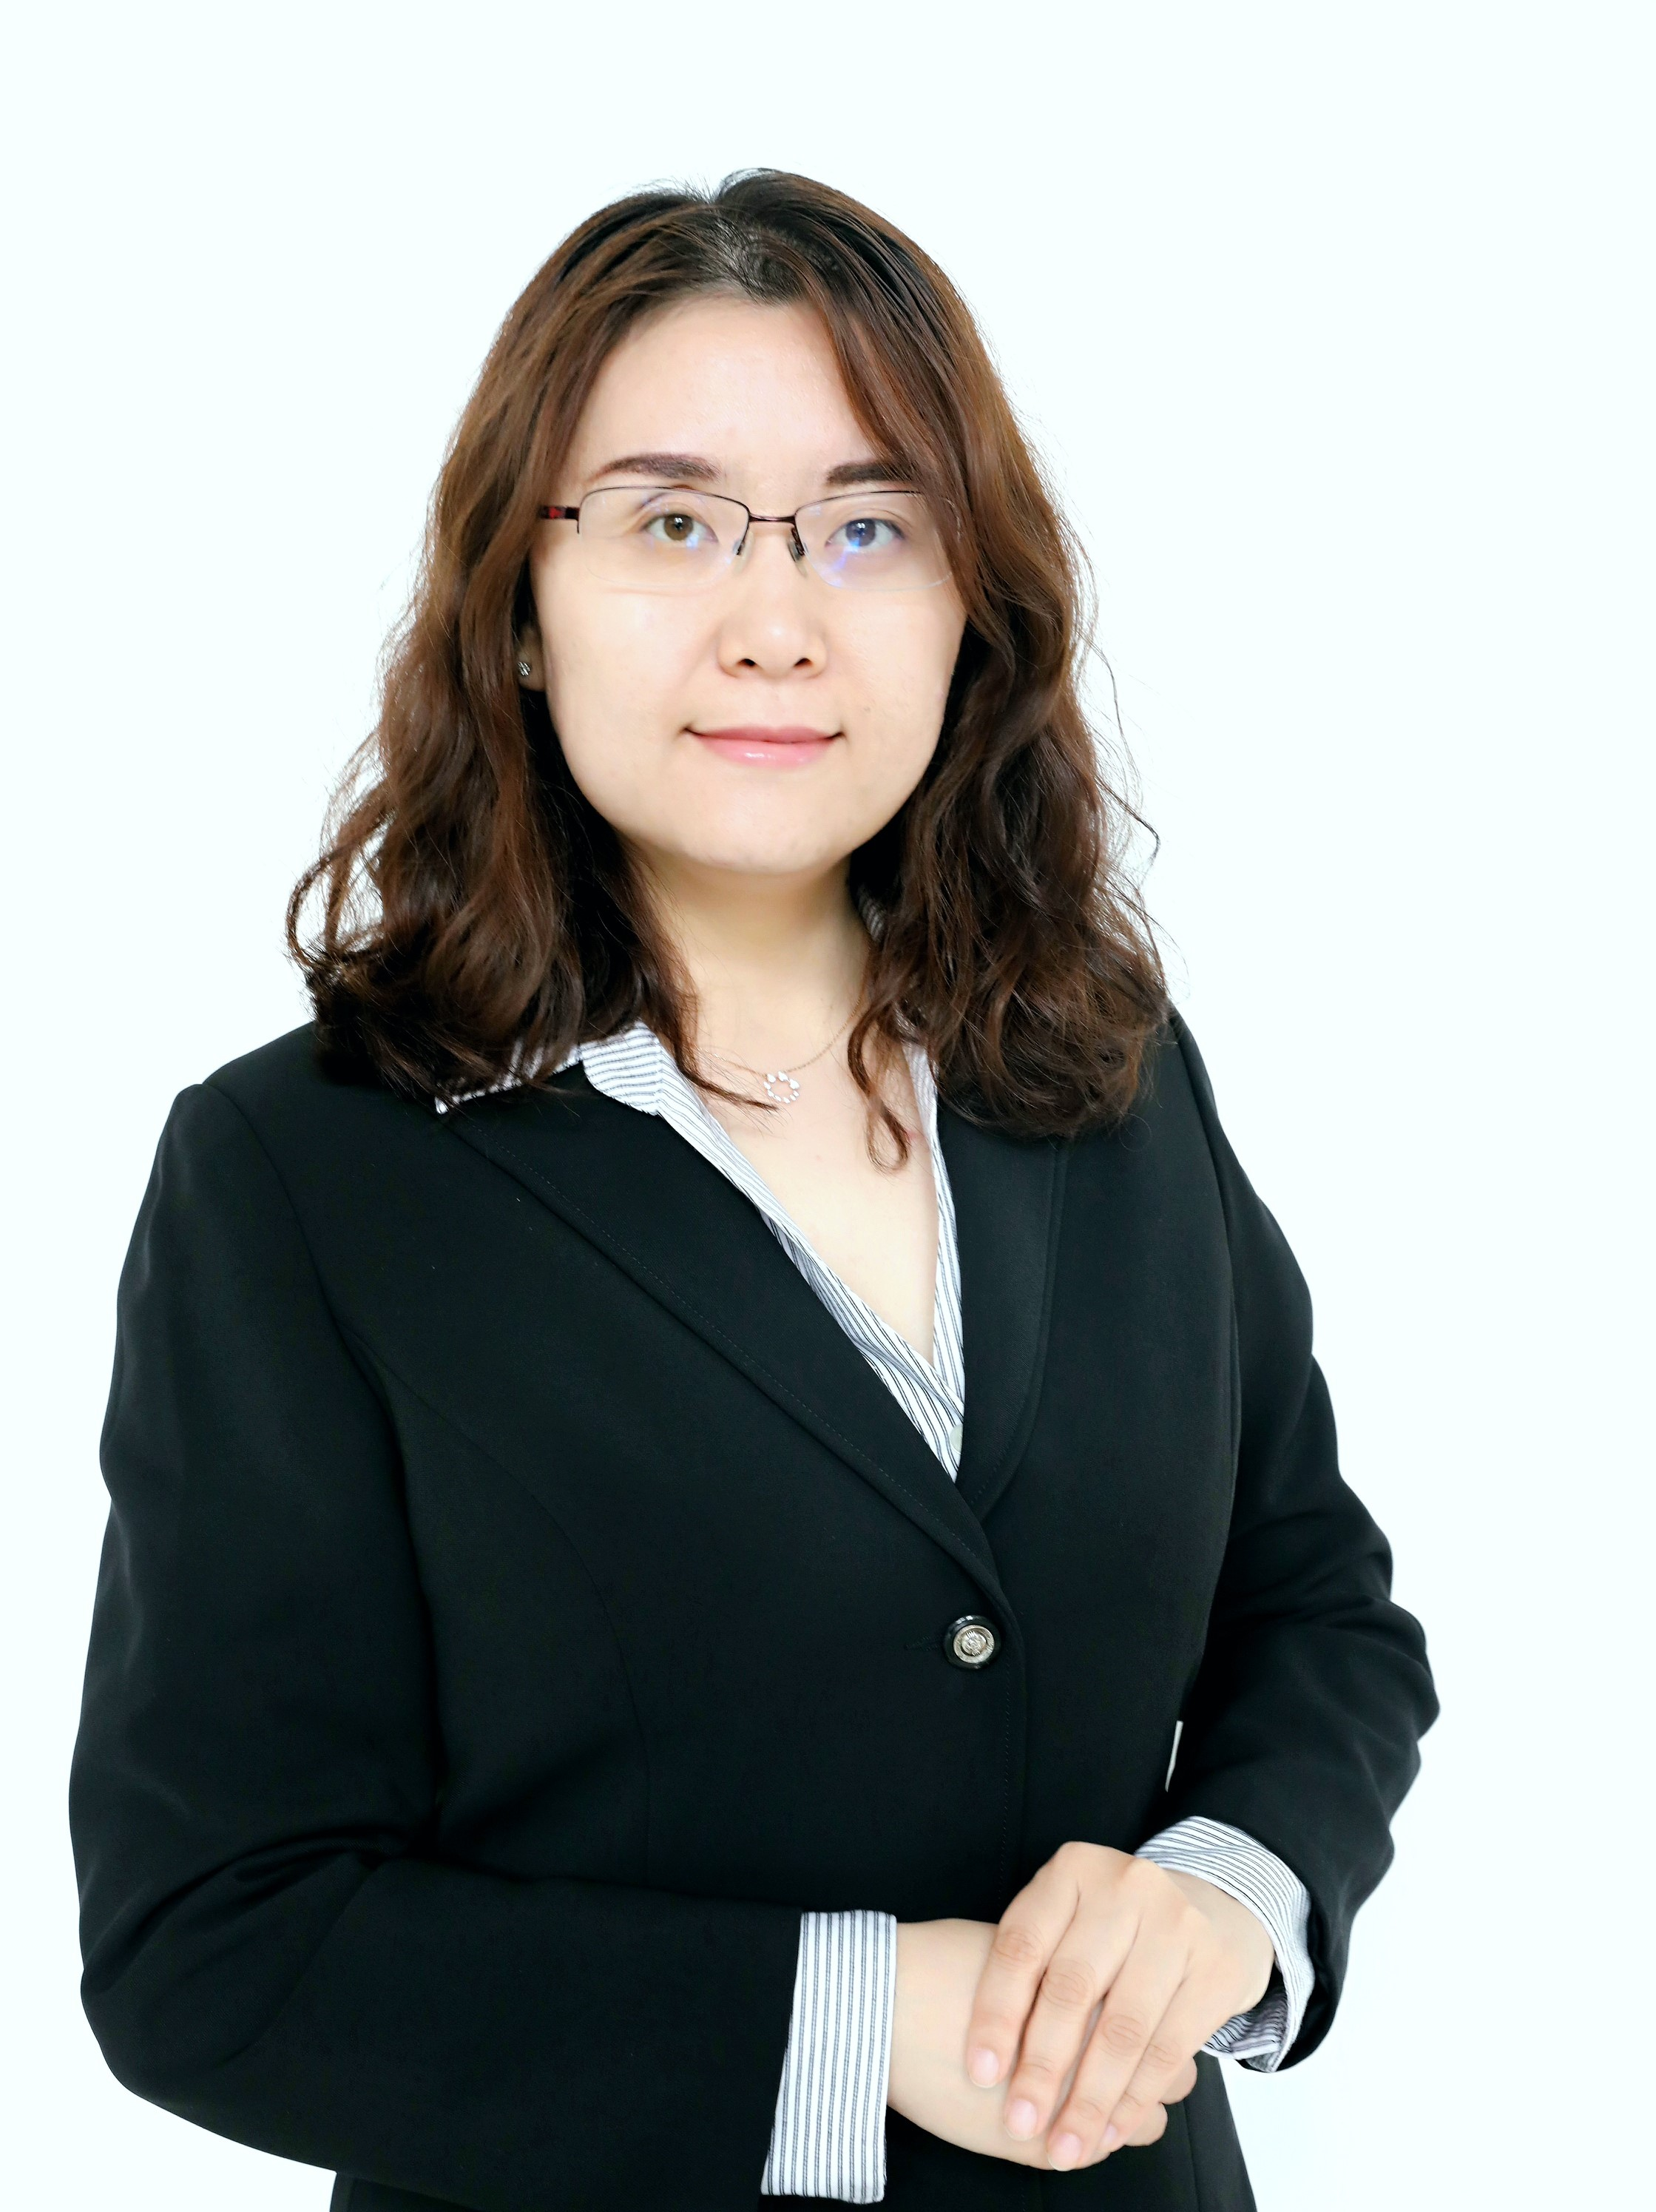
\includegraphics[width=1in,height=1.25in,clip,keepaspectratio]{figure/Gao.jpg}}]{Xiaofeng Gao}
(Senior Member, IEEE) received the B.S. degree from Nankai University, China, in 2004, the M.S. degree from Tsinghua University, China, in 2006, and the Ph.D. degree from The University of Texas at Dallas, USA, in 2010. She is currently a Full Professor with the School of Computer Science, Shanghai Jiao Tong University, China. Her research interests include data engineering and network optimizations. She has published over 150 peer-reviewed papers in the related area, including well-archived international journals, such as the IEEE TRANSACTIONS ON COMPUTERS, IEEE TRANSACTIONS ON KNOWLEDGE AND DATA ENGINEERING, IEEE TRANSACTIONS ON MOBILE COMPUTING, IEEE TRANSACTIONS ON PARALLEL AND DISTRIBUTED SYSTEMS, and also in well-known conference proceedings, such as SIGKDD, INFOCOM, WWW, ICDE, etc. She has served on the Editorial Board of Discrete Mathematics, Algorithms, and Applications.
\end{IEEEbiography}

\begin{IEEEbiography}[{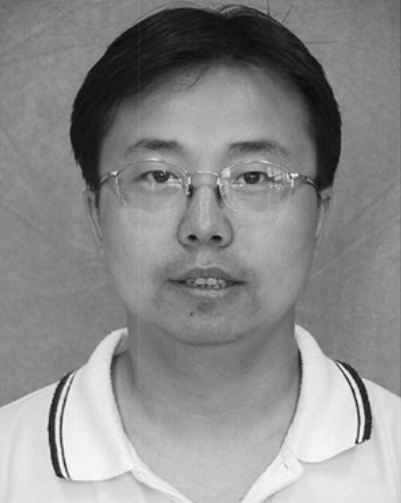
\includegraphics[width=1in,height=1.25in,clip,keepaspectratio]{figure/binwang.png}}]{Bin Wang} received the Ph.D. degree in computer science and technology from Northeastern University, Shenyang, China, in 2008. He is currently a Professor with the School of Computer Science and Engineering, Northeastern University. His research interests include big data management and knowledge engineering, database theory and technology, cloud computing, and data privacy preserving. More details about his research can be found at http://faculty.neu.edu.cn/wangbin.
\end{IEEEbiography}

\begin{IEEEbiography}
[{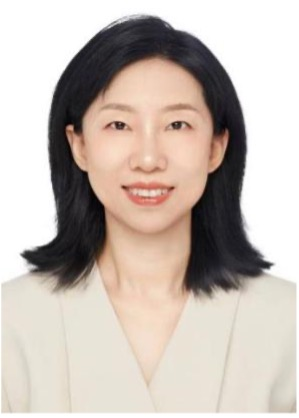
\includegraphics[width=1in,height=1.25in,clip,keepaspectratio]{figure/xiaochunyang.jpg}}]{Xiaochun Yang} 
(Senior Member, IEEE) received the Ph.D. degree in computer software and theory from Northeastern University, Shenyang, China, in 2001. She is currently a Professor with the Software College, Northeastern University. Her research interests include big data management and knowledge engineering, data quality management, data privacy preserving, and recommender systems. For more information visit the link (http://faculty.neu.edu.cn/yangxiaochun).
\end{IEEEbiography}

\begin{IEEEbiography}
[{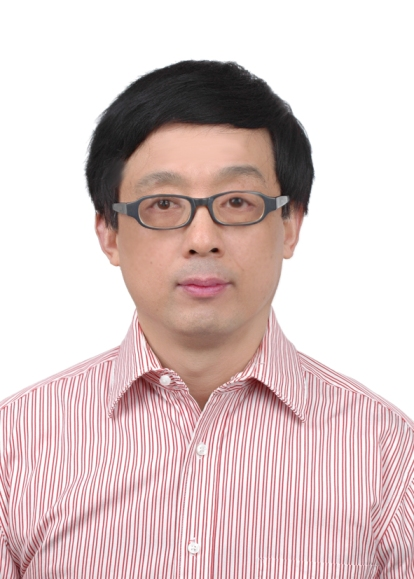
\includegraphics[width=1in,height=1.25in,clip,keepaspectratio]{figure/chen.jpg}}]{Guihai Chen}
(Fellow, IEEE) is a distinguished professor of Shanghai Jiao Tong University. He had been invited as a visiting professor by the Kyushu Institute of Technology, Japan, University of Queensland, Australia and Wayne State University. He has a wide range of research interests with focus on parallel computing, wireless networks, data centers, peer-to-peer computing, high-performance computer architecture and data engineering. He has published more than 350 peer-reviewed papers, and more than 200 of them are in well-archived international journals such as IEEE Transactions on Parallel and Distributed Systems, IEEE Transactions on Computers and IEEE/ACM Transactions on Networking, and also in well-known conference proceedings such as SIGCOMM, MobiCom, OSDI, ICNP, INFOCOM, CoNEXT and AAAI. He has won nine best paper awards including ICNP 2015 best paper award and DASFAA 2017 best paper award. He is a fellow of CCF.
\end{IEEEbiography}

\end{document}


\subsection{Lists}
In this section, we will consider three types of lists: simple unnumbered, numbered, and bulleted. There have been many options added to IEEEtran to enhance the creation of lists. If your lists are more complex than those shown below, please refer to the original ``IEEEtran\_HOWTO.pdf'' for additional options.\\

\subsubsection*{\bf A plain  unnumbered list}
\begin{list}{}{}
\item{bare\_jrnl.tex}
\item{bare\_conf.tex}
\item{bare\_jrnl\_compsoc.tex}
\item{bare\_conf\_compsoc.tex}
\item{bare\_jrnl\_comsoc.tex}
\end{list}

\subsubsection*{\bf A simple numbered list}
\begin{enumerate}
\item{bare\_jrnl.tex}
\item{bare\_conf.tex}
\item{bare\_jrnl\_compsoc.tex}
\item{bare\_conf\_compsoc.tex}
\item{bare\_jrnl\_comsoc.tex}
\end{enumerate}

\subsubsection*{\bf A simple bulleted list}
\begin{itemize}
\item{bare\_jrnl.tex}
\item{bare\_conf.tex}
\item{bare\_jrnl\_compsoc.tex}
\item{bare\_conf\_compsoc.tex}
\item{bare\_jrnl\_comsoc.tex}
\end{itemize}





\subsection{Figures}
Fig. 1 is an example of a floating figure using the graphicx package.
 Note that $\backslash${\tt{label}} must occur AFTER (or within) $\backslash${\tt{caption}}.
 For figures, $\backslash${\tt{caption}} should occur after the $\backslash${\tt{includegraphics}}.

\begin{figure}[!t]
\centering
\includegraphics[width=2.5in]{fig1}
\caption{Simulation results for the network.}
\label{fig_1}
\end{figure}

Fig. 2(a) and 2(b) is an example of a double column floating figure using two subfigures.
 (The subfig.sty package must be loaded for this to work.)
 The subfigure $\backslash${\tt{label}} commands are set within each subfloat command,
 and the $\backslash${\tt{label}} for the overall figure must come after $\backslash${\tt{caption}}.
 $\backslash${\tt{hfil}} is used as a separator to get equal spacing.
 The combined width of all the parts of the figure should do not exceed the text width or a line break will occur.
%
\begin{figure*}[!t]
\centering
\subfloat[]{\includegraphics[width=2.5in]{fig1}%
\label{fig_first_case}}
\hfil
\subfloat[]{\includegraphics[width=2.5in]{fig1}%
\label{fig_second_case}}
\caption{Dae. Ad quatur autat ut porepel itemoles dolor autem fuga. Bus quia con nessunti as remo di quatus non perum que nimus. (a) Case I. (b) Case II.}
\label{fig_sim}
\end{figure*}

Note that often IEEE papers with multi-part figures do not place the labels within the image itself (using the optional argument to $\backslash${\tt{subfloat}}[]), but instead will
 reference/describe all of them (a), (b), etc., within the main caption.
 Be aware that for subfig.sty to generate the (a), (b), etc., subfigure
 labels, the optional argument to $\backslash${\tt{subfloat}} must be present. If a
 subcaption is not desired, leave its contents blank,
 e.g.,$\backslash${\tt{subfloat}}[].


 

\section{Tables}
Note that, for IEEE-style tables, the
 $\backslash${\tt{caption}} command should come BEFORE the table. Table captions use title case. Articles (a, an, the), coordinating conjunctions (and, but, for, or, nor), and most short prepositions are lowercase unless they are the first or last word. Table text will default to $\backslash${\tt{footnotesize}} as
 the IEEE normally uses this smaller font for tables.
 The $\backslash${\tt{label}} must come after $\backslash${\tt{caption}} as always.
 
\begin{table}[!t]
\caption{An Example of a Table\label{tab:table1}}
\centering
\begin{tabular}{|c||c|}
\hline
One & Two\\
\hline
Three & Four\\
\hline
\end{tabular}
\end{table}

\section{Algorithms}
Algorithms should be numbered and include a short title. They are set off from the text with rules above and below the title and after the last line.

\begin{algorithm}[H]
\caption{Weighted Tanimoto ELM.}\label{alg:alg1}
\begin{algorithmic}
\STATE 
\STATE {\textsc{TRAIN}}$(\mathbf{X} \mathbf{T})$
\STATE \hspace{0.5cm}$ \textbf{select randomly } W \subset \mathbf{X}  $
\STATE \hspace{0.5cm}$ N_\mathbf{t} \gets | \{ i : \mathbf{t}_i = \mathbf{t} \} | $ \textbf{ for } $ \mathbf{t}= -1,+1 $
\STATE \hspace{0.5cm}$ B_i \gets \sqrt{ \textsc{max}(N_{-1},N_{+1}) / N_{\mathbf{t}_i} } $ \textbf{ for } $ i = 1,...,N $
\STATE \hspace{0.5cm}$ \hat{\mathbf{H}} \gets  B \cdot (\mathbf{X}^T\textbf{W})/( \mathbb{1}\mathbf{X} + \mathbb{1}\textbf{W} - \mathbf{X}^T\textbf{W} ) $
\STATE \hspace{0.5cm}$ \beta \gets \left ( I/C + \hat{\mathbf{H}}^T\hat{\mathbf{H}} \right )^{-1}(\hat{\mathbf{H}}^T B\cdot \mathbf{T})  $
\STATE \hspace{0.5cm}\textbf{return}  $\textbf{W},  \beta $
\STATE 
\STATE {\textsc{PREDICT}}$(\mathbf{X} )$
\STATE \hspace{0.5cm}$ \mathbf{H} \gets  (\mathbf{X}^T\textbf{W} )/( \mathbb{1}\mathbf{X}  + \mathbb{1}\textbf{W}- \mathbf{X}^T\textbf{W}  ) $
\STATE \hspace{0.5cm}\textbf{return}  $\textsc{sign}( \mathbf{H} \beta )$
\end{algorithmic}
\label{alg1}
\end{algorithm}

Que sunt eum lam eos si dic to estist, culluptium quid qui nestrum nobis reiumquiatur minimus minctem. Ro moluptat fuga. Itatquiam ut laborpo rersped exceres vollandi repudaerem. Ulparci sunt, qui doluptaquis sumquia ndestiu sapient iorepella sunti veribus. Ro moluptat fuga. Itatquiam ut laborpo rersped exceres vollandi repudaerem. 
\section{Mathematical Typography \\ and Why It Matters}

Typographical conventions for mathematical formulas have been developed to {\bf provide uniformity and clarity of presentation across mathematical texts}. This enables the readers of those texts to both understand the author's ideas and to grasp new concepts quickly. While software such as \LaTeX \ and MathType\textsuperscript{\textregistered} can produce aesthetically pleasing math when used properly, it is also very easy to misuse the software, potentially resulting in incorrect math display.

IEEE aims to provide authors with the proper guidance on mathematical typesetting style and assist them in writing the best possible article. As such, IEEE has assembled a set of examples of good and bad mathematical typesetting \cite{ref1,ref2,ref3,ref4,ref5}. 

Further examples can be found at \url{http://journals.ieeeauthorcenter.ieee.org/wp-content/uploads/sites/7/IEEE-Math-Typesetting-Guide-for-LaTeX-Users.pdf}

\subsection{Display Equations}
The simple display equation example shown below uses the ``equation'' environment. To number the equations, use the $\backslash${\tt{label}} macro to create an identifier for the equation. LaTeX will automatically number the equation for you.
\begin{equation}
\label{deqn_ex1}
x = \sum_{i=0}^{n} 2{i} Q.
\end{equation}

\noindent is coded as follows:
\begin{verbatim}
\begin{equation}
\label{deqn_ex1}
x = \sum_{i=0}^{n} 2{i} Q.
\end{equation}
\end{verbatim}

To reference this equation in the text use the $\backslash${\tt{ref}} macro. 
Please see (\ref{deqn_ex1})\\
\noindent is coded as follows:
\begin{verbatim}
Please see (\ref{deqn_ex1})\end{verbatim}

\subsection{Equation Numbering}
{\bf{Consecutive Numbering:}} Equations within an article are numbered consecutively from the beginning of the
article to the end, i.e., (1), (2), (3), (4), (5), etc. Do not use roman numerals or section numbers for equation numbering.

\noindent {\bf{Appendix Equations:}} The continuation of consecutively numbered equations is best in the Appendix, but numbering
 as (A1), (A2), etc., is permissible.\\

\noindent {\bf{Hyphens and Periods}}: Hyphens and periods should not be used in equation numbers, i.e., use (1a) rather than
(1-a) and (2a) rather than (2.a) for subequations. This should be consistent throughout the article.

\subsection{Multi-Line Equations and Alignment}
Here we show several examples of multi-line equations and proper alignments.

\noindent {\bf{A single equation that must break over multiple lines due to length with no specific alignment.}}
\begin{multline}
\text{The first line of this example}\\
\text{The second line of this example}\\
\text{The third line of this example}
\end{multline}

\noindent is coded as:
\begin{verbatim}
\begin{multline}
\text{The first line of this example}\\
\text{The second line of this example}\\
\text{The third line of this example}
\end{multline}
\end{verbatim}

\noindent {\bf{A single equation with multiple lines aligned at the = signs}}
\begin{align}
a &= c+d \\
b &= e+f
\end{align}
\noindent is coded as:
\begin{verbatim}
\begin{align}
a &= c+d \\
b &= e+f
\end{align}
\end{verbatim}

The {\tt{align}} environment can align on multiple  points as shown in the following example:
\begin{align}
x &= y & X & =Y & a &=bc\\
x' &= y' & X' &=Y' &a' &=bz
\end{align}
\noindent is coded as:
\begin{verbatim}
\begin{align}
x &= y & X & =Y & a &=bc\\
x' &= y' & X' &=Y' &a' &=bz
\end{align}
\end{verbatim}





\subsection{Subnumbering}
The amsmath package provides a {\tt{subequations}} environment to facilitate subnumbering. An example:

\begin{subequations}\label{eq:2}
\begin{align}
f&=g \label{eq:2A}\\
f' &=g' \label{eq:2B}\\
\mathcal{L}f &= \mathcal{L}g \label{eq:2c}
\end{align}
\end{subequations}

\noindent is coded as:
\begin{verbatim}
\begin{subequations}\label{eq:2}
\begin{align}
f&=g \label{eq:2A}\\
f' &=g' \label{eq:2B}\\
\mathcal{L}f &= \mathcal{L}g \label{eq:2c}
\end{align}
\end{subequations}

\end{verbatim}

\subsection{Matrices}
There are several useful matrix environments that can save you some keystrokes. See the example coding below and the output.

\noindent {\bf{A simple matrix:}}
\begin{equation}
\begin{matrix}  0 &  1 \\ 
1 &  0 \end{matrix}
\end{equation}
is coded as:
\begin{verbatim}
\begin{equation}
\begin{matrix}  0 &  1 \\ 
1 &  0 \end{matrix}
\end{equation}
\end{verbatim}

\noindent {\bf{A matrix with parenthesis}}
\begin{equation}
\begin{pmatrix} 0 & -i \\
 i &  0 \end{pmatrix}
\end{equation}
is coded as:
\begin{verbatim}
\begin{equation}
\begin{pmatrix} 0 & -i \\
 i &  0 \end{pmatrix}
\end{equation}
\end{verbatim}

\noindent {\bf{A matrix with square brackets}}
\begin{equation}
\begin{bmatrix} 0 & -1 \\ 
1 &  0 \end{bmatrix}
\end{equation}
is coded as:
\begin{verbatim}
\begin{equation}
\begin{bmatrix} 0 & -1 \\ 
1 &  0 \end{bmatrix}
\end{equation}
\end{verbatim}

\noindent {\bf{A matrix with curly braces}}
\begin{equation}
\begin{Bmatrix} 1 &  0 \\ 
0 & -1 \end{Bmatrix}
\end{equation}
is coded as:
\begin{verbatim}
\begin{equation}
\begin{Bmatrix} 1 &  0 \\ 
0 & -1 \end{Bmatrix}
\end{equation}\end{verbatim}

\noindent {\bf{A matrix with single verticals}}
\begin{equation}
\begin{vmatrix} a &  b \\ 
c &  d \end{vmatrix}
\end{equation}
is coded as:
\begin{verbatim}
\begin{equation}
\begin{vmatrix} a &  b \\ 
c &  d \end{vmatrix}
\end{equation}\end{verbatim}

\noindent {\bf{A matrix with double verticals}}
\begin{equation}
\begin{Vmatrix} i &  0 \\ 
0 & -i \end{Vmatrix}
\end{equation}
is coded as:
\begin{verbatim}
\begin{equation}
\begin{Vmatrix} i &  0 \\ 
0 & -i \end{Vmatrix}
\end{equation}\end{verbatim}

\subsection{Arrays}
The {\tt{array}} environment allows you some options for matrix-like equations. You will have to manually key the fences, but there are other options for alignment of the columns and for setting horizontal and vertical rules. The argument to {\tt{array}} controls alignment and placement of vertical rules.

A simple array
\begin{equation}
\left(
\begin{array}{cccc}
a+b+c & uv & x-y & 27\\
a+b & u+v & z & 134
\end{array}\right)
\end{equation}
is coded as:
\begin{verbatim}
\begin{equation}
\left(
\begin{array}{cccc}
a+b+c & uv & x-y & 27\\
a+b & u+v & z & 134
\end{array} \right)
\end{equation}
\end{verbatim}

A slight variation on this to better align the numbers in the last column
\begin{equation}
\left(
\begin{array}{cccr}
a+b+c & uv & x-y & 27\\
a+b & u+v & z & 134
\end{array}\right)
\end{equation}
is coded as:
\begin{verbatim}
\begin{equation}
\left(
\begin{array}{cccr}
a+b+c & uv & x-y & 27\\
a+b & u+v & z & 134
\end{array} \right)
\end{equation}
\end{verbatim}

An array with vertical and horizontal rules
\begin{equation}
\left( \begin{array}{c|c|c|r}
a+b+c & uv & x-y & 27\\ \hline
a+b & u+v & z & 134
\end{array}\right)
\end{equation}
is coded as:
\begin{verbatim}
\begin{equation}
\left(
\begin{array}{c|c|c|r}
a+b+c & uv & x-y & 27\\
a+b & u+v & z & 134
\end{array} \right)
\end{equation}
\end{verbatim}
Note the argument now has the pipe "$\vert$" included to indicate the placement of the vertical rules.


\subsection{Cases Structures}
Many times cases can be miscoded using the wrong environment, i.e., {\tt{array}}. Using the {\tt{cases}} environment will save keystrokes (from not having to type the $\backslash${\tt{left}}$\backslash${\tt{lbrace}}) and automatically provide the correct column alignment.
\begin{equation*}
{z_m(t)} = \begin{cases}
1,&{\text{if}}\ {\beta }_m(t) \\ 
{0,}&{\text{otherwise.}} 
\end{cases}
\end{equation*}
\noindent is coded as follows:
\begin{verbatim}
\begin{equation*}
{z_m(t)} = 
\begin{cases}
1,&{\text{if}}\ {\beta }_m(t),\\ 
{0,}&{\text{otherwise.}} 
\end{cases}
\end{equation*}
\end{verbatim}
\noindent Note that the ``\&'' is used to mark the tabular alignment. This is important to get  proper column alignment. Do not use $\backslash${\tt{quad}} or other fixed spaces to try and align the columns. Also, note the use of the $\backslash${\tt{text}} macro for text elements such as ``if'' and ``otherwise.''

\subsection{Function Formatting in Equations}
Often, there is an easy way to properly format most common functions. Use of the $\backslash$ in front of the function name will in most cases, provide the correct formatting. When this does not work, the following example provides a solution using the $\backslash${\tt{text}} macro:

\begin{equation*} 
  d_{R}^{KM} = \underset {d_{l}^{KM}} {\text{arg min}} \{ d_{1}^{KM},\ldots,d_{6}^{KM}\}.
\end{equation*}

\noindent is coded as follows:
\begin{verbatim}
\begin{equation*} 
 d_{R}^{KM} = \underset {d_{l}^{KM}} 
 {\text{arg min}} \{ d_{1}^{KM},
 \ldots,d_{6}^{KM}\}.
\end{equation*}
\end{verbatim}

\subsection{ Text Acronyms Inside Equations}
This example shows where the acronym ``MSE" is coded using $\backslash${\tt{text\{\}}} to match how it appears in the text.

\begin{equation*}
 \text{MSE} = \frac {1}{n}\sum _{i=1}^{n}(Y_{i} - \hat {Y_{i}})^{2}
\end{equation*}

\begin{verbatim}
\begin{equation*}
 \text{MSE} = \frac {1}{n}\sum _{i=1}^{n}
(Y_{i} - \hat {Y_{i}})^{2}
\end{equation*}
\end{verbatim}

\section{Conclusion}
The conclusion goes here.


\section*{Acknowledgments}
This should be a simple paragraph before the References to thank those individuals and institutions who have supported your work on this article.



{\appendix[Proof of the Zonklar Equations]
Use $\backslash${\tt{appendix}} if you have a single appendix:
Do not use $\backslash${\tt{section}} anymore after $\backslash${\tt{appendix}}, only $\backslash${\tt{section*}}.
If you have multiple appendixes use $\backslash${\tt{appendices}} then use $\backslash${\tt{section}} to start each appendix.
You must declare a $\backslash${\tt{section}} before using any $\backslash${\tt{subsection}} or using $\backslash${\tt{label}} ($\backslash${\tt{appendices}} by itself
 starts a section numbered zero.)}



%{\appendices
%\section*{Proof of the First Zonklar Equation}
%Appendix one text goes here.
% You can choose not to have a title for an appendix if you want by leaving the argument blank
%\section*{Proof of the Second Zonklar Equation}
%Appendix two text goes here.}



\section{References Section}
You can use a bibliography generated by BibTeX as a .bbl file.
 BibTeX documentation can be easily obtained at:
 http://mirror.ctan.org/biblio/bibtex/contrib/doc/
 The IEEEtran BibTeX style support page is:
 http://www.michaelshell.org/tex/ieeetran/bibtex/
 
 % argument is your BibTeX string definitions and bibliography database(s)
%\bibliography{IEEEabrv,../bib/paper}
%
\section{Simple References}
You can manually copy in the resultant .bbl file and set second argument of $\backslash${\tt{begin}} to the number of references
 (used to reserve space for the reference number labels box).

\begin{thebibliography}{1}
\bibliographystyle{IEEEtran}

\bibitem{ref1}
{\it{Mathematics Into Type}}. American Mathematical Society. [Online]. Available: https://www.ams.org/arc/styleguide/mit-2.pdf

\bibitem{ref2}
T. W. Chaundy, P. R. Barrett and C. Batey, {\it{The Printing of Mathematics}}. London, U.K., Oxford Univ. Press, 1954.

\bibitem{ref3}
F. Mittelbach and M. Goossens, {\it{The \LaTeX Companion}}, 2nd ed. Boston, MA, USA: Pearson, 2004.

\bibitem{ref4}
G. Gr\"atzer, {\it{More Math Into LaTeX}}, New York, NY, USA: Springer, 2007.

\bibitem{ref5}M. Letourneau and J. W. Sharp, {\it{AMS-StyleGuide-online.pdf,}} American Mathematical Society, Providence, RI, USA, [Online]. Available: http://www.ams.org/arc/styleguide/index.html

\bibitem{ref6}
H. Sira-Ramirez, ``On the sliding mode control of nonlinear systems,'' \textit{Syst. Control Lett.}, vol. 19, pp. 303--312, 1992.

\bibitem{ref7}
A. Levant, ``Exact differentiation of signals with unbounded higher derivatives,''  in \textit{Proc. 45th IEEE Conf. Decis.
Control}, San Diego, CA, USA, 2006, pp. 5585--5590. DOI: 10.1109/CDC.2006.377165.

\bibitem{ref8}
M. Fliess, C. Join, and H. Sira-Ramirez, ``Non-linear estimation is easy,'' \textit{Int. J. Model., Ident. Control}, vol. 4, no. 1, pp. 12--27, 2008.

\bibitem{ref9}
R. Ortega, A. Astolfi, G. Bastin, and H. Rodriguez, ``Stabilization of food-chain systems using a port-controlled Hamiltonian description,'' in \textit{Proc. Amer. Control Conf.}, Chicago, IL, USA,
2000, pp. 2245--2249.

\end{thebibliography}


\newpage

\section{Biography Section}
If you have an EPS/PDF photo (graphicx package needed), extra braces are
 needed around the contents of the optional argument to biography to prevent
 the LaTeX parser from getting confused when it sees the complicated
 $\backslash${\tt{includegraphics}} command within an optional argument. (You can create
 your own custom macro containing the $\backslash${\tt{includegraphics}} command to make things
 simpler here.)
 
\vspace{11pt}

\bf{If you include a photo:}\vspace{-33pt}
\begin{IEEEbiography}[{\includegraphics[width=1in,height=1.25in,clip,keepaspectratio]{fig1}}]{Michael Shell}
Use $\backslash${\tt{begin\{IEEEbiography\}}} and then for the 1st argument use $\backslash${\tt{includegraphics}} to declare and link the author photo.
Use the author name as the 3rd argument followed by the biography text.
\end{IEEEbiography}

\vspace{11pt}

\bf{If you will not include a photo:}\vspace{-33pt}
\begin{IEEEbiographynophoto}{John Doe}
Use $\backslash${\tt{begin\{IEEEbiographynophoto\}}} and the author name as the argument followed by the biography text.
\end{IEEEbiographynophoto}

\vfill

\end{document}


